\documentclass[11pt,spanish]{report}

% Margins (optional tweak)
\usepackage[a4paper,left=1.18in,right=1in,top=1in,bottom=1in]{geometry}

\usepackage{dsfont}

% IEEE style bibliography
\usepackage[backend=biber,style=ieee]{biblatex}
\addbibresource{refs.bib}


% Language and font
\usepackage[spanish]{babel}
\usepackage[utf8]{inputenc}
\usepackage[T1]{fontenc}
\usepackage{fontspec}
\setmainfont{Arial}


\usepackage{amsmath,amssymb}
\usepackage{graphicx}
\usepackage{url}
% \usepackage{cite}
\usepackage{hyperref}
\usepackage{caption}
\usepackage{subcaption}
\usepackage[dvipsnames]{xcolor} 


\usepackage{hyperref}
\hypersetup{
        colorlinks=true,            
        linkcolor=Blue,               
        citecolor=blue,                          
        urlcolor=blue,
        bookmarksdepth=4
}

\usepackage{slashed}
\usepackage{titlesec}
\usepackage{tocloft}  % Para personalizar las listas de tablas                % ---------- May, 10th
\usepackage{paracol}  % Más flexible que parcolumns

% Double spacing
\usepackage{setspace}
\doublespacing

% Page formatting
\usepackage{fancyhdr}
\pagestyle{fancy}
\fancyhf{} % Clear default header/footer
\fancyfoot[R]{\thepage} % Page number bottom-right
\renewcommand{\headrulewidth}{0pt} % No header line
\renewcommand{\footrulewidth}{0pt} % No footer line

% Page numbering for frontmatter and mainmatter
\usepackage{etoolbox}
\makeatletter
\patchcmd{\chapter}{\thispagestyle{plain}}{\thispagestyle{mychapterstyle}}{}{}
\makeatother

% Custom page style for chapters (roman numbering, non-plain)
\fancypagestyle{mychapterstyle}{
  \fancyhf{}
  \fancyfoot[R]{\thepage}
}

% Custom page style for plain pages (arabic numbering)
\fancypagestyle{plain}{
  \fancyhf{}
  \fancyfoot[R]{\thepage}
}

% Roman numbering for frontmatter, Arabic for mainmatter
\newcommand{\frontmatter}{
  \pagenumbering{roman}
  \renewcommand{\thepage}{\roman{page}}
}
\newcommand{\mainmatter}{
  \cleardoublepage
  \pagenumbering{arabic}
}


% ORCID
\newcommand{\orcid}[1]{\href{https://orcid.org/#1}{\includegraphics[width=8pt]{orcid.pdf}}}


\usepackage{caption}
\captionsetup[table]{name=Tabla} % Cambia "Cuadro" → "Tabla" en el cuerpo del documento, no en la Lista de Tablas


% Capítulos en 14 pt
\titleformat{\chapter}
  {\normalfont\fontsize{14pt}{16pt}\bfseries}
  {\thechapter}{1em}{}

% Secciones (subcapítulos) en 11 pt
\titleformat{\section}
  {\normalfont\fontsize{11pt}{13pt}\bfseries}
  {\thesection}{1em}{}

% Sangria 0.5 pulgadas
\setlength{\parindent}{0.5in}


\addto\captionsspanish{\renewcommand{\contentsname}{\hspace{2in} \Large Tabla de Contenido}}


\renewcommand{\thesection}{\Alph{section}.} % Muestra A, B, C (sin "II.")
\renewcommand{\thesubsection}{\arabic{subsection}} % 1, 2, 3...


\renewcommand{\thefigure}{\Roman{figure}}
\renewcommand{\cftfigpresnum}{Figura~}
\renewcommand{\cftfigaftersnum}{:}
\counterwithout{figure}{chapter}
\setlength{\cftfignumwidth}{5em}
% Formato en el caption de las figuras
\captionsetup[figure]{labelformat=simple, labelsep=colon}


\renewcommand{\thechapter}{\Roman{chapter}} % I, II, III...


\titleformat{\chapter}[display]
  {\Large\bfseries\centering}
  {}
  {0pt}
  {}




\newcommand{\listappendixname}{Lista de Anexos}
\newlistof{appendix}{loa}{\listappendixname}
\renewcommand{\cftappendixpresnum}{Anexo~}  % Optional: Prefix entries with "Anexo"







\begin{document}

\frontmatter

\begin{titlepage}
\thispagestyle{empty}
    \centering
    \vspace*{1cm}

    {\Large \textbf{UNIVERSIDAD NACIONAL DE INGENIERIA}}\\[1.25cm]

    {\Large \textbf{Facultad de Ciencias}}\\[1.25cm]

{\includegraphics[scale = 0.25]{Images/logo_UNI.png}} \\ 
    \vspace{0.4cm}
    
	TESIS 
	
	\vspace{0.1in}
    
    { \Large \textbf{Materia oscura en el modelo $\nu_R-$331}}\\[0.5cm]
%\chapter*{Anexos}
	
	Para obtener el Título Profesional de Licenciado en Física	\\

	Elaborado por \\

    Guillermo Gerardo Rivera Gambini \\ \orcid{0000-0002-9381-7049} ORCID: 0000-0002-9381-7049  \\
    
	Asesor  \\
    
    Dr. Oscar Eduardo Castillo Ruiz \\ \orcid{0000-0001-9713-6040} ORCID: 0000-0001-9713-6040  \\[1.0cm]


    \vfill
    \textbf{LIMA$-$PERÚ}\\
    2025

\end{titlepage}
\setcounter{page}{2} % Fuerza a que la próxima página sea "ii"



\noindent\rule{16cm}{0.6pt}
\vspace{-0.4in}
\setcolumnwidth{0.3\textwidth, 0.7\textwidth}
\begin{paracol}{2}

\switchcolumn* 
\noindent Rivera Gambini [1]

\noindent [1] \hspace{0.2in} G. Rivera Gambini, ``Materia oscura en el modelo \\ \indent $\nu_R-331$'' [Tesis de pregrado]. Lima (Perú): Universidad \\ \indent Nacional de Ingenieria, 2025.

\switchcolumn

\centering

Citar/How to cite \\

\vspace{-0.2in}
\noindent\rule{4.5cm}{0.6pt}
\vspace{-0.6in}
\noindent Referencia/Reference


\end{paracol}
\vspace{-0.2in}
\noindent\rule{16cm}{0.6pt}



\vspace{1in}


\noindent\rule{16cm}{0.6pt}
\vspace{-0.4in}
\setcolumnwidth{0.3\textwidth, 0.7\textwidth}
\begin{paracol}{2}

\switchcolumn* 
\noindent (Rivera, 2025)

\noindent Rivera, G. (2025), Materia oscura en el modelo $\nu_R-331$ \\ \indent [Tesis de pregrado, Universidad Nacional de \\ \indent Ingenieria]. Repositorio Institucional UNI.

\switchcolumn

\centering

Citar/How to cite \\

\vspace{-0.2in}
\noindent\rule{4.5cm}{0.6pt}
\vspace{-0.6in}
\noindent Referencia/Reference

\end{paracol}
\vspace{-0.2in}
\noindent\rule{16cm}{0.6pt}

\newpage


\chapter*{\hfill \textit{Dedicatoria}}

\begin{flushright}
\textit{Dedico este trabajo a mi mamá, a mi abuelo, a mi hermana y a mis hermanos, que siempre han estado ahí para apoyarme.}
\end{flushright}


\chapter*{Agradecimientos}
En primer lugar, me gustaría agradecer a mi familia por su infinita paciencia y constante apoyo a mis proyectos.

En seguida me gustaria agradecer a mi asesor el Dr. Oscar Eduardo Castillo Ruiz, al Dr. Orlando L. Pereyra Ravinez y al Dr. Rosendo Ochoa por su guía y tutoría después de tantos años de haber egresado de la UNI.

Me gustaría agradecer a Jim Cline y a Farilando Queiroz a quienes les debo gran parte de lo que he aprendido a lo largo de estos años.  

No podrían faltar los amigos que están presente dentro y fuera del mundo académico. Entre ellos tenemos a Fernanda de Faria Rodrigues, Gabriel Rabelo Soares, Lucia Angel, Armando Pezo, Dennis Zavaleta, Marvyn Inga, Fiorella Aquino, Lis Corbacho y Caroline Mouls.

\chapter*{Resumen}
\addcontentsline{toc}{chapter}{\protect\numberline{}Resumen} % Añade a TOC sin número
El modelo estándar de física de partículas, a pesar de su notable éxito, no logra dar cuenta de la existencia de materia oscura, un componente fundamental del presupuesto energético del universo. Los modelos $3-3-1$, basados en el grupo de gauge $SU(3)_C \times SU(3)_L \times U(1)_X$, proporcionan un marco convincente para abordar varias preguntas abiertas en física de partículas, incluida la naturaleza de la materia oscura. En esta tesis, exploramos la viabilidad de un candidato de materia oscura dentro del modelo $\nu_R-$331, una realización específica del marco $3-3-1$ que acomoda naturalmente un candidato de materia oscura estable WIMP. Específicamente, analizamos las restricciones fenomenológicas sobre la abundancia de reliquias de materia oscura resolviendo la ecuación de Boltzmann para diferentes canales de interacción entre la materia oscura y las partículas del modelo estándar. Nuestros resultados demuestran que un candidato viable de materia oscura puede surgir naturalmente dentro de este modelo, ofreciendo una alternativa atractiva a las extensiones convencionales del modelo estándar.

\  \

\noindent
\textbf{Keywords:} materia oscura, modelo 331, WIMP, fenomenología


\chapter*{Abstract}
\addcontentsline{toc}{chapter}{\protect\numberline{}Abstract} % Añade a TOC sin número
%\addcontentsline{toc}{chapter}{Abstract}
The standard model of particle physics, despite its remarkable success, fails to account for the existence of dark matter, a fundamental component of the universe's energy budget. The $3-3-1$ models, based on the gauge group 
$SU(3)_C \times SU(3)_L \times U(1)_X$ , provide a compelling framework to address various open questions in particle physics, including the nature of dark matter. In this thesis, we explore the viability of a dark matter candidate within the $\nu_R-$331 model, a specific realization of the $3-3-1$ framework that naturally accommodates a stable WIMP dark matter candidate. Specifically, we analyze the phenomenological constraints on the dark matter relic abundance by solving the Boltzmann equation for different interaction channels between dark matter and standard model particles. Our results demonstrate that a viable dark matter candidate can naturally arise within this model, offering an attractive alternative to conventional extensions of the standard model.

\  \ 

\noindent
\textbf{Keywords:} dark matter, 331 model, WIMP, phenomenology




\clearpage
\tableofcontents

\clearpage
\renewcommand{\listtablename}{\hspace{2.4in} \Large Lista de Tablas}
\renewcommand{\thetable}{\Roman{table}} % I, II, III...
\listoftables
%%%%%\renewcommand{\tablename}{Tablaaaa}


\clearpage
\renewcommand{\listfigurename}{\hspace{2.4in} \Large Lista de Figuras}
\renewcommand{\thefigure}{\Roman{figure}}
\listoffigures


\chapter*{Índice de acrónimos}
\begin{center}
%{\huge Índice de Acrónimos}\\[2cm]
\end{center}
\bigskip
\begin{tabular}{ l c l }

\textbf{ME} & & Modelo Estándar\\
\textbf{LHC} & & Large Hadron Collider\\
\textbf{LEP} & & Large Electron-Positron Collider\\
\textbf{CERN} & & Conseil Européen pour la Recherche nucléaire\\
\textbf{FCNC} & & Flavor Changing Neutral Current\\
\textbf{SSB} & & Spontaneous Symmetry Breaking\\
\textbf{WIMP} & & Weakly Interacting Massive Particle\\ 
\textbf{DM} & & Dark Matter \\
\textbf{NFW} & & Navarro-Frenk-White\\
\textbf{H.E.S.S.} & & High Energy Stereoscopic System \\
\textbf{CTA} & & Cherenkov Telescope Array \\
\end{tabular}


% MAINMATTER
\mainmatter

% ===============
% C H A P T E R S 
% ===============
\chapter*{Introducción}
\addcontentsline{toc}{chapter}{\protect\numberline{}Introducción} % Añade a TOC sin número
Comprender el universo donde vivimos siempre ha sido de gran interés para la humanidad. Cerca de 200 a.C., el sabio griego Eratóstenes de Cirene pudo determinar la longitud de la circunferencia de la Tierra al contratar un profesional que midió la distancia entre Siena y Alejandría y hallar el ángulo de inclinación de la sombra de un palo fijado en el suelo en Alejandría al medio dia el dia del solsticio de verano cuando la sombra era nula en Siena.

En esa época en la antigua Grecia ya existía la teoría filosófica del Atomismo según la cual pequeñas partículas indivisibles, llamadas átomos, componen el universo. Sin embargo, no es hasta finales del sigo XVIII que John Dalton propuso una teoría atómica moderna donde los átomos se usan para explicar los diferentes elementos químicos y sus reacciones. En esta teoría los diferentes tipos de átomos seguían siendo considerados indivisibles.

Más adelante, a finales del siglo XIX, la teoría atómica cambiaría con los experimentos de J. J. Thomson quien propuso que los átomos tienen estructura. Así, creó su modelo atómico donde el átomo es una esfera cargada positivamente y en ella se encuentran distribuidos los electrones de manera tal que el conjunto total sea eléctricamente nulo. 

Al descubrir el núcleo atómico, Ernest Rutherford creó un nuevo modelo para el átomo donde el núcleo era una pequeña región densa cargada positivamente y los electrones orbitan alrededor de ella. El modelo mejoró posteriormente con el descubrimiento de los neutrones por parte de James Chadwick. Actualmente se entiende que el núcleo atómico está formado por protones y neutrones.

Con la invención de la teoría de la relatividad especial de Einstein, la mecánica cuántica  y su unión en la teoría cuántica de campos a inicios del siglo XX, se pudieron sentar las bases matemáticas rigurosas para entender mejor la estructura del átomo y sus interacciones. Se entendió que existen tres tipos de interacciones cuánticas: la electrodinámica que mantiene a los electrones `alrededor' del núcleo, la interacción fuerte que mantiene al núcleo unido a si mismo y la interacción débil que permite la transformación del núcleo en uno de otro tipo.

A finales de los años 1970 se había construido una teoría que era capaz de explicar todos los experimentos en física de partículas a la fecha: el modelo estándar de la física de partículas. Aquí, los protones y neutrones se entienden como compuestos de quarks unidos por la `fuerza' nuclear fuerte que acabamos de mencionar. 


La última pieza del `rompecabezas' del modelo estándar era el bosón de Higgs que fue propuesto en 1964 y descubierto en el CERN en 2012 por las colaboraciones ATLAS \cite{ATLAS:2012yve} y CMS \cite{CMS:2012qbp}. El bosón de Higgs es la partícula del campo de Higgs y tiene carga eléctrica neutra, tiempo de vida corto y spin cero. Sus interacciones con el leptón tau y el quark top fueron medidas en 2016 y 2018, respectivamente. Esto último es interesante porque el tau y el top son los fermiones más pesados del modelo estándar y por eso son los que interactúan más fuertemente con el campo de Higgs: \textit{mientras más fuerte sea la interacción con el campo de Higgs, mayor será la masa de dicha partícula}.

Existe, sin embargo, una partícula que aparentemente no interacciona con el campo de Higgs. Esta partícula es el neutrino, el cual tiene masa nula en la teoría del modelo estándar. Esta partícula viene en tres `sabores': electrónico, muónico y tauónico, y tienen la asombrosa propiedad de oscilar entre esos sabores. Este fenómeno llamado de \textit{oscilación de neutrinos} es posible solo cuando los neutrinos tienen masa y estas son diferentes una de la otra. 

Esta aparente contradicción con el mecanismo de generación de masa por medio de la interacción con el campo de Higgs puede desaparecer postulando nuevas partículas que acoplan con los neutrinos y el Higgs. Estas partículas tendrían que ser muy pesadas en comparación con las energías de los experimentos terrestres ya que no han sido detectadas. Se puede decir que, de existir, estas partículas pertenecerían a un sector oscuro, diferente del modelo estándar.

La idea de un sector oscuro no es nueva. A inicios del siglo XX, observaciones astronómicas permitieron concluir que hay un tipo de materia no lumínica la cual no se ha podido detectar directamente pero su influencia gravitacional está presente (y es dominante) en las galáxias y los cúmulos de galáxias. Es así como nace la propuesta de \textit{materia oscura}, un nuevo (o nuevos) tipo(s) de materia que no es descrita por partículas del modelo estándar.

En este trabajo estudiaremos la materia oscura en una extensión del modelo estándar llamada \textit{modelos} $3-3-1$ \cite{PhysRevD.46.410}. Estos modelos son ricos en nuevas partículas e interacciones, lo que es deseable para hacer fenomenología de altas energías. Estos modelos han sido exitosos en, por ejemplo, explicar que el número de familias fermiónicas sea igual a tres \cite{Foot:1992rh} y la cuantización de la carga eléctrica \cite{deSousaPires:1998jc}. En particular, nos enfocaremos en el modelo $\nu_R$-331 \cite{Singer:1980sw} y calcularemos la densidad de relíquia para un candidato a materia oscura dada por un escalar complejo con masa desde los cientos de GeV hasta decenas de TeV. 

%En este trabajo analizamos límites experimentales de detección indirecta de materia oscura para un escalar complejo proveniente de una extensión del modelo estándar llamada \textit{modelos} $3-3-1$. En estos modelos se postula la existencia de más de un campo escalar `tipo Higgs', los cuales son necesários para reproducir los resultados del modelo estándar a `bajas energías' con unas pequeñas correcciones. En particular, nos enfocaremos en el modelo $3-3-1$ Económico y usaremos límites experimentales obtenidos por la colaboración H.E.S.S. que investiga rayos gamma usando telescópios atmosféricos de tipo Cherenkov.  


\color{black}

\chapter[\hspace{-0.185in}.  El Modelo Estándar]{I. El Modelo Estándar}
El propósito de este capítulo es definir el modelo estándar rápidamente, enfocándonos en el sector electrodébil, y mostrar que ha sobrevivido muchas pruebas experimentales. Esto hace del modelo estándar una teoría excelente, válida en un amplio rango de energías y el límite al cual otras teorías `más allá del modelo estándar' deberían aproximarse a `bajas energías'.

\section[\hspace{-0.14in}Introducción]{Introducción}

A finales de la década de 1970, el Modelo Estándar (ME) de la física de partículas, creado por Weinberg, Salam y Glashow, comenzó a consolidarse como la teoría básica de la materia. Aquí los constituyentes fundamentales son partículas de spin $1/2$ y son llamados \textit{quarks} y \textit{leptones}. Estas interacciones entre partículas es mediada por otras partículas de spin $0$ (el bosón de Higgs) y $1$ (fotones, gluones y los bosones W y Z) \cite{Weinberg:1967tq}. 


Hasta una década antes del ME, se pensaba que los protones, neutrones, piones, kaones y otras partículas que interactuaban fuertemente (hadrones) eran elementales. Sin embargo, el consenso que surgió más adelante fue que los hadrones estaban compuestos de bloques más básicos llamados quarks y se mantenían unidos mediante el intercambio de gluones \cite{hoddeson1992rise}.

En la figura \ref{SMparticles} podemos ver los seis sabores $f$ para los quarks, es decir, $f= u$ (arriba), $d$ (abajo), $c$ (encantado), $s$ (extraño), $t$  (cima) y $b$ (fondo) en rosado, los seis leptones: el electrón (e), el muón ($\mu$) y el tau ($\tau$), más sus neutrinos asociados ($\nu_e, \nu_{\mu}, \nu_{\tau}$) en verde, y los portadores de fuerza: el fotón ($\gamma$), el gluón (g) y los bosones Z y W en anaranjado. Finalmente, en amarillo tenemos el bosón de Higgs el cual está separado de los otros bosones por no ser un bosón de gauge. Esto último quiere decir que no está asociado al grupo de gauge del ME, $SU(3)_C \times SU(2)_L \times U(1)_Y$, donde $C,L,Y$ representan color, quiralidad izquierda e hipercarga, respectivamente. 

\begin{figure}[!h]
\centering
\includegraphics[width=7cm]{Images/SM-particles.pdf}
\caption[Campos cuánticos del Modelo Estándar]{El ME explica cómo los componentes básicos de la materia (los quarks y los leptones) interactúan a través de tres de las cuatro fuerzas fundamentales.}
\label{SMparticles}
\end{figure}


\section[\hspace{-0.175in} El sector electrodébil]{El sector electrodébil}

Las partículas del ME ganan masa por medio del mecanismo de Higgs, el cual es una realización de la quiebra espontánea de la simetría, $SU(2)_L \times U(1)_Y \rightarrow U(1)_Q$, donde $Q$ es la carga eléctrica. En la tabla \ref{table1} podemos ver los números cuánticos del contenido de matéria del ME donde $I$ es el isospín débil e $I_3$ es su tercera componente. La carga eléctrica se calcula a partir de la relación Gell-Mann$-$Nishijima $Q=I_3 + Y/2$. 


\begin{table}[h]
\caption[\hspace{-0.15in}Números cuánticos del Modelo Estándar]{Números cuánticos electrodébiles de los fermiones en el modelo estándar. Las tres generaciones de los quarks y los letones están representadas por un solo símbolo $Q$ y $L$ para los dobletes de $SU(2)_L$ y $q_R,\ell_R$ para los singletos. Los subíndices $L$ y $R$ denotan quiralidad izquierda y derecha, respectivamente.}
\begin{center}
\begin{small}
\begin{tabular}{|c | c | c | c | c|} 
 \hline
 Representaciones irreducibles & & & & \\ fermiónicas de $SU(2)_L \times U(1)_Y$ & $I$ & $I_3$ & $Y$ & $Q$ \\ [1ex] 
 \hline\hline
 $L \equiv 
	\begin{pmatrix}
	\nu \\
	\ell 
	\end{pmatrix}_L $ & $1/2$ & $\begin{array}{c} 1/2 \\ \hspace{-0.1in} -1/2 \end{array}$	 & \hspace{-0.1in} $-1$ & $0$ \\ 
[1ex]
 \hline
 $\ell_R$ & $0$ & $0$ & \hspace{-0.1in} $-2$ & $1$ \\ [0.25ex] 
 \hline
  $Q \equiv 
	\begin{pmatrix}
	u \\
	d 
	\end{pmatrix}_L $ & $1/2$ & $\begin{array}{c} 1/2 \\ \hspace{-0.1in} -1/2 \end{array}$	 & $1/3$ & $\begin{array}{c} 2/3 \\ \hspace{-0.1in} -1/3 \end{array}$ \\ 
[1ex]
 \hline
  $u_R$ & $0$ & $0$ & $4/3$ & $2/3$ \\ [0.25ex] 
 \hline
 $d_R$ & $0$ & $0$ & \hspace{-0.1in} $-2/3$ & \hspace{-0.1in} $ -1/3$ \\ [0.25ex] 
 \hline
\end{tabular}
\end{small}
\label{table1}
\end{center}
\end{table}


Con la simetría gauge del ME y el contenido de matéria verificado experimentalmente podemos construir la lagrangeana del sector electrodébil,
\begin{eqnarray}
\mathcal{L} &=& i \overline{L} \slashed{D} L + i \overline{Q} \slashed{D} Q + i \overline{\ell_R} \slashed{D} \ell_R +  i \overline{u_R} \slashed{D} u_R + i \overline{d_R} \slashed{D} d_R  \nonumber \\
            &-& \frac{1}{4} \vec{F}^{\mu \nu} \cdot \vec{F}_{\mu \nu} -\frac{1}{4}B_{\mu \nu} B^{\mu \nu} \nonumber \\
             &+&\left(D_\rho \Phi \right)^\dagger \left( D^\rho \Phi \right) + \mu^2 \Phi^\dagger \Phi - \lambda \left( \Phi^\dagger \Phi \right)^2 \nonumber \\
             &-& \left[ Y^{\ell}\, \overline{L}\Phi \ell + Y^{u}\, \overline{Q}(-i\sigma_2 \Phi^*) u + Y^{d}\, \overline{Q}\Phi d  + H.c.  \right],
\end{eqnarray}
donde la derivada covariante es $D_\mu \equiv \partial_\mu + ig\vec{A}_\mu \cdot\vec{\sigma}/2 +ig' B_\mu Y/2$ y tanto $\vec{A}_\mu$ como $B_\mu$ son bosones de gauge de los grupos $SU(2)_L$ y $U(1)_Y$, respectivamente, $\sigma_2$ es la segunda matriz de Pauli y $\Phi$ es el doblete de Higgs cuyos números cuánticos son mostrados en la tabla \ref{table2}

\begin{table}[h]
\caption{\hspace{-0.15in}Números cuánticos electrodébiles para el doblete de Higgs.}
\begin{center}
\begin{small}
\begin{tabular}{|c | c | c | c | c|} 
 \hline
Doblete de Higgs & $I$ & $I_3$ & $Y$ & $Q$ \\ [1ex] 
 \hline\hline
 $\Phi \equiv 
	\begin{pmatrix}
	\phi^+ \\
	\phi^0 
	\end{pmatrix} $ & $1/2$ & $\begin{array}{c} 1/2 \\ \hspace{-0.1in} -1/2 \end{array}$	 & $1$ & $\begin{array}{c} 1 \\ 0 \end{array}$ \\ 
[1ex]
 \hline
\end{tabular}
\end{small}
\label{table2}
\end{center}
\end{table}

 Cabe notar que los neutrinos no son las únicas partículas del ME que permanecen sin masa después del rompimiento espontáneo de simetría. Los fotones y los gluones también permanecen no masivos, pero a diferencia de los neutrinos, esto se debe a que $SU(3)_C \times U(1)_Q$ permanece como una simetría del ME después de la quiebra de simetría. Este mistério  relacionado al origen de las masas de los neutrinos es física está más allá del ME es una de las áreas de investigación más activas actualmente.



\section[\hspace{-0.19in} Tests del modelo estándar]{Tests del modelo estándar}

A lo largo de su história, el modelo estándar ha probado que funciona muy bien al superar varias pruebas. En esta sección comentaremos un poco sobre algunos de esos tests, básicamente aquellos que fueron hechos en el CERN\footnote{Conseil Européen pour la Recherche nucléaire $-$ Consejo Europeo para la Investigación Nuclear.}.

El gran colisionador de electrones y positrones LEP\footnote{Large Electron-Positron collider \href{https://home.cern/science/accelerators/large-electron-positron-collider}{LEP}.} en el CERN operó de 1989 al 2000. Este acelerador circular contaba con un anillo de aproximadamenteo 27 km y habían cuatro detectores multipropósito: L3, ALEPH, OPAL y DELPHI (ver figura \ref{LEPmap}).

\begin{figure}[h]
\centering
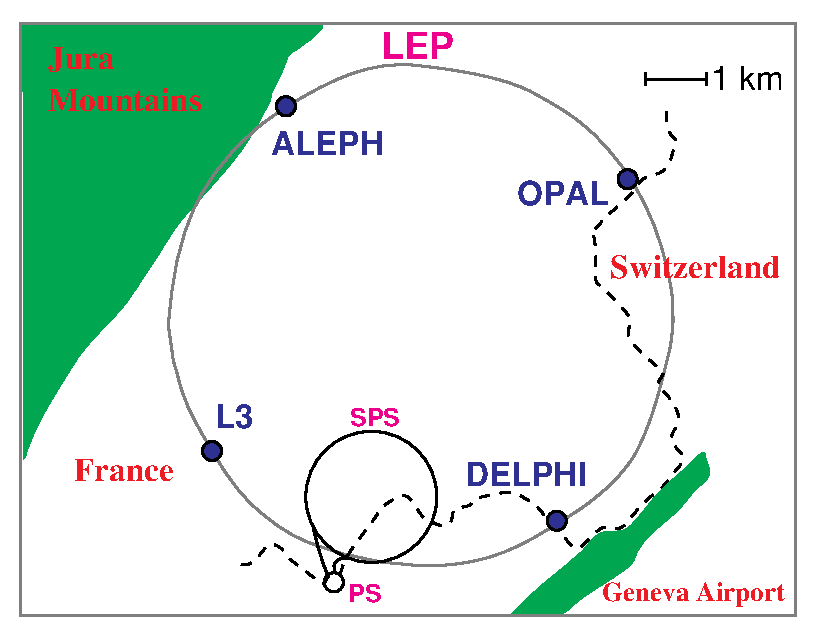
\includegraphics[scale=0.8]{Images/lep_map.eps}
\caption[Mapa del Large Electron-Positron Collider (LEP)]{Mapa del Large Electron-Positron Collider (LEP) \cite{aleph2005precision}.}
\label{LEPmap}
\end{figure}

Al final de la toma de datos con energias del centro de masa alrededor de la resonancia del bosón Z, cerca de 1000 bosones Z eran registrados cada hora por cada uno de los cuatro experimentos previamente mencionados. Esto hizo de LEP una fábrica de bosones Z y algunos de sus resultados fueron:
\begin{itemize}
	\item \textbf{La resonancia del bosón Z:} La sección de choque de la colisión $e^+e^-$ sufre un incremento de cerca de 3 ordenes de magnitud cuando la energía del centro de masa alcanza la masa del bosón Z, $m_Z$. Esto se debe a que el bosón Z acopla con todos los fermiones de manera similar a los fotones. Aparece entonces un competidor para este último al momento de mediar dicha interacción. Para energías abajo de $\sim 40$ GeV, el fotón domina. A energías mayores ambos son igual de importanes, pero cerca de la resonancia del bosón Z, este domina. Esto se entiende en el ME debido a que la amplitud total del proceso es $\mathcal{M}=\mathcal{M}_\gamma+\mathcal{M}_Z$, $\mathcal{M}_\gamma\propto 1/q^2 $, $\mathcal{M}_Z \propto 1/[q^2 -m_Z^2 + im_Z\Gamma_Z]$, $\Gamma_Z$ es el ancho de decaimiento del bosón Z, siendo la sección total de choque es proporcional a $|\mathcal{M}|^2=|\mathcal{M}_\gamma+\mathcal{M}_Z|^2$. De esta manera, cada mediador tiene su región donde domina pero también existen regiones donde interfieren y ninguno lo hace (ver la figura \ref{SMt1}).
	
	
\begin{figure}[h!]
\centering
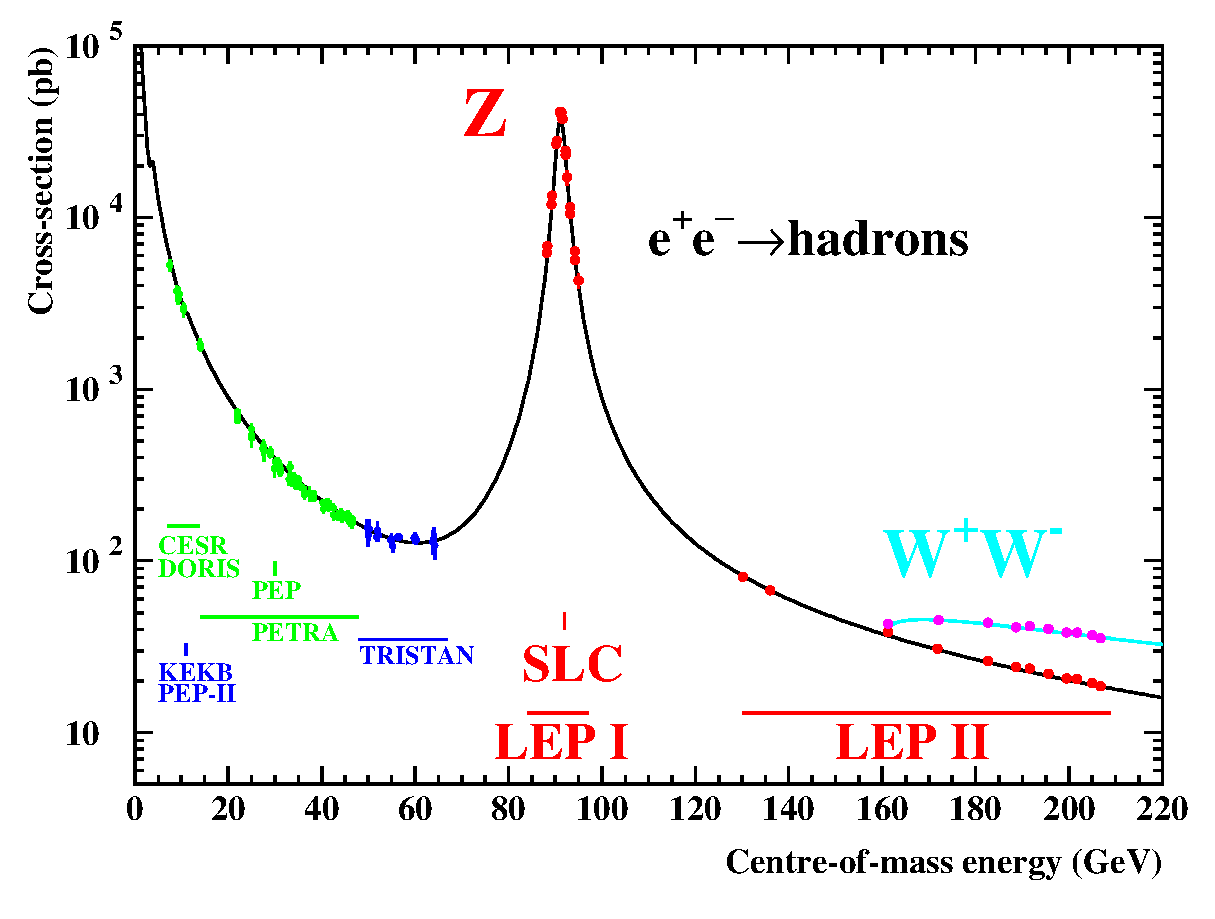
\includegraphics[scale=0.55]{Images/SM-test-1.eps}
\caption[Sección de choque hadrónica en la resonancia del boson Z]{Sección de choque hadrónica en la resonancia del boson Z \cite{aleph2005precision}. El pico en la sección de choque para $e^+e^-\to$ hadrons cerca de $\sim$90 GeV no se puede explicar con la electrodinámica cuántica (QED). El bosón Z del ME puede explicar este aumento.}
\label{SMt1}
\end{figure}
	
\newpage	
	\item \textbf{El ancho de decaimiento del bosón Z:} Aunque los neutrinos no sean observados en los experimentos previamente mencionados, ellos afectan significativamente el ancho de decaimiento del bosón Z, esto es \cite{thomson2013modern}
	\begin{equation}
	\Gamma_Z = 3\Gamma_{\ell \ell} + \Gamma_{\rm hadrons} + n_\nu\Gamma_{\nu\nu},
	\end{equation}	  
	asumiendo universalidad leptónica\footnote{Esto quiere decir que las diferentes generaciones de leptones acoplan de la misma manera con los bosones de gauge.}. 
	
En la figura \ref{SMt2} se muestra que $n_\nu =3$ da el mejor ajuste a los datos combinados de los cuatro experimentos. Este resultado está de acuerdo con otros resultados experimentales independientes como, por ejemplo, el número efectivo de neutrinos $N_{\rm eff}=2.99(17)$ obtenidos del estudio del fondo cósmico de microondas (CMB)\footnote{Ver el siguiente capítulo.} hecho por la colaboración Planck \cite{aghanim2020planck}. Sin embargo, podría existir otros `neutrinos' más pesados que no pueden ser producidos en los decaimientos del bosón Z y no afectan el número de especies relativísticas del universo en el momento de la formación del CMB.
	
\begin{figure}[h!]
\centering
\includegraphics[scale=0.55]{Images/SM-test-2.eps}
  \caption[Sección de choque variando con el número de neutrinos]{Sección de choque variando con el número de neutrinos \cite{aleph2005precision}. Mediciones del ancho de decaimiento del bosón Z concuerdan con la predicción del ME cuando el número de neutrinos activos es 3. Actualmente no se han observado más de tres de estos neutrinos ni sus respectivos leptones a los que asociados.}
  \label{SMt2}
\end{figure}
	
	
\newpage	
	
\item \textbf{Masa de los bosones W:} En LEP, a diferencia del bosón Z, la masas de los bosones W son obtenidas de la producción de pares $W^+W^-$. Cerca de $\sqrt{s}=2\,m_W$, la sección de choque $\sigma (e^+e^- \to W^+W^-)$ depende fuertemente de $m_W$ y $\Gamma_W$ ya que los W están \textit{on-shell}\footnote{Esto quiere decir que cumplen $E^2=m^2+p^2$.}, pero para energías del centro de masa $\sqrt{s}$ mayores, se debe reconstruir las masas invariantes de los productos finales considerando a los bosones $W$ tanto \textit{on-shell} como virtuales (ver figura \ref{eeWW}).
\begin{figure}[h]
\centering
\includegraphics[scale=0.45]{Images/ee_to_WW.pdf}
\caption[Diagrama de Feynman para $e^+e^- \to W^+W^-$ con estado final $qq\ell \nu$]{Diagrama de Feynman para $e^+e^- \to W^+W^-$ con estado final de tipo $qq\ell \nu$. La colaboración L3 analizó estados finales conteniendo cuatro fermiones: $\ell \nu\ell \nu$, $qq\ell \nu$ y $qqqq$.}
\label{eeWW}
\end{figure}

%La colaboración L3 analizó estados finales conteniendo cuatro fermiones: $\ell \nu\ell \nu$, $qq\ell \nu$ y $qqqq$. En la figura \ref{eeWW} podemos ver el diagrama de Feynman para un proceso donde las masas invariantes $m_1^2=(p_\nu + p_\ell)^2$ y $m_2^2=(p_{\bar{q}}+p_q)^2$ son diferentes. 


\  \

En la figura \ref{SMt3} podemos ver esta sección de choque $\sigma (e^+e^- \to W^+W^-)$ medida a $\sqrt{s}=$ 161 GeV \cite{acciarri1997pair}, 172 GeV \cite{acciarri1997measurement}, 183 GeV \cite{acciarri1998measurement} y valores mayores \cite{achard2004measurement}. Cuando los bosones $W$ son virtuales, sus masas mudan en cada evento y son, en general, distintas entre sí. La figura \ref{SMt4} muestra la distribución del promedio de estas masas para los eventos $e^+e^- \to W^{+}W^{-}\to q\bar{q}\ell \nu$. Los resultados de las simulaciones Monte Carlo del ME están muy de acuerdo con estos dos resultados experimentales\footnote{Recientemente la colaboración CDF anunció una medida de la masa del W que discrepa con la predicción del ME \cite{cdf2022high}. Este resultado se aleja de los valores reportados por otros experimentos los cuales también son muy precisos y están de acuerdo con el ME.}. 
\end{itemize}


\begin{figure}[h!]
\centering
\includegraphics[scale=0.35]{Images/SM-test-6.pdf}
\caption[Sección de choque de $e^+e^- \to W^+W^-$]{Sección de choque de $e^+e^- \to W^+W^-$ \cite{achard2004measurement}. Los resultados experimentales para la sección de choque para $e^+e^- \to W^+W^-$ concuerdan con la predicción del ME.}
\label{SMt3}
\end{figure}

\begin{figure}[h!]
\centering
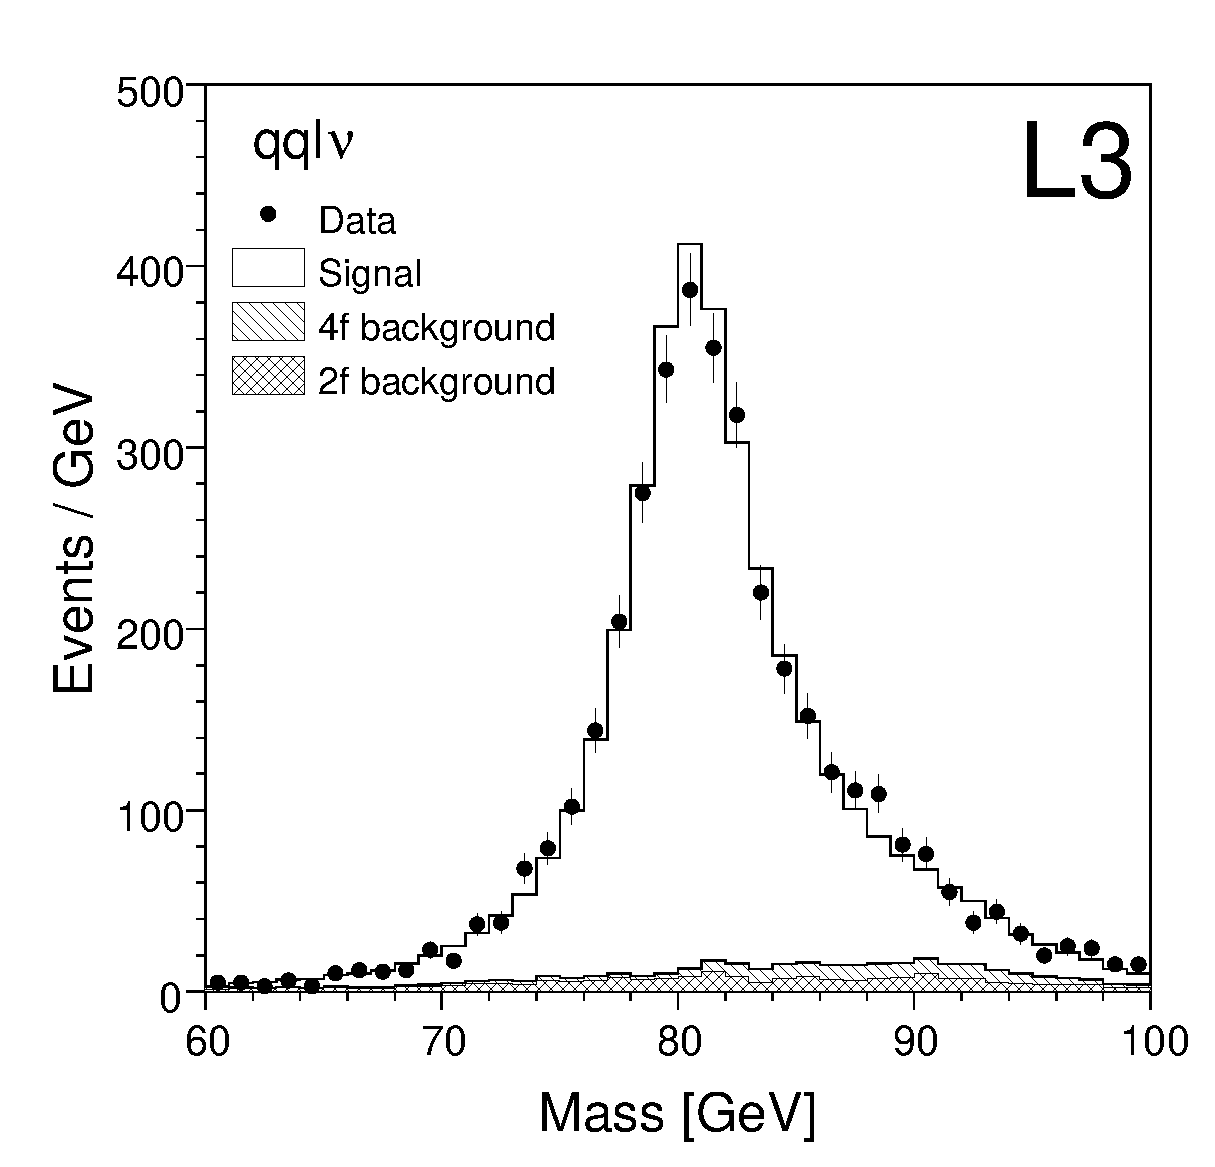
\includegraphics[scale=0.4]{Images/SM-test-3.eps}
\caption[Distribución de masas reconstruidas del bosón W]{Distribución de masas reconstruidas del bosón W \cite{l32006measurement}. La distribución de la masa del W concuerda con las simulaciones Monte Carlo en el contexto del ME.}
 \label{SMt4}
\end{figure}



\begin{itemize}
	\item \textbf{Asimetría forward-backward:} Los productos de la colisión $e^+e^-$ mediados por un bosón Z (por ejemplo, $e^+e^- \to Z^* \to \mu^+\mu^-$, ver figura \ref{eeZmumu}) aparecen haciendo un ángulo $\theta$ con relación al eje de los haces iniciales. 
\begin{figure}[h]
\centering
\includegraphics[scale=0.2]{Images/A_FB.png}
\caption[Par $\mu^+\mu^-$ producido en la colisión $e^+e^-$]{Par $\mu^+\mu^-$ producido en la colisión $e^+e^-$ \cite{thomson2013modern}.}
\label{eeZmumu}
\end{figure}	
	
	Esta distribución no es isotrópica en el ME ya que los acoplamientos del bosón Z con fermiones de mano derecha e izquierda son diferentes. Por ejemplo, para el proceso $e^+e^- \to Z^* \to \mu^+\mu^-$ tenemos (ignorando contribuciones de la QED cerca de $\sqrt{s}\sim m_Z$),
\[
\mathcal{M} = - \frac{g_z^2}{s-m_Z^2+i m_Z \Gamma_Z} g_{\mu \nu}\bigg[ \bar{v} \gamma^\mu \frac{1}{2} \left( c_V^e -c_A^e \gamma^5 \right) u \bigg] \bigg[ \bar{u} \gamma^\mu \frac{1}{2} \left( c_V^\mu -c_A^\mu \gamma^5 \right) v \bigg]
\]
y de ahí se obtiene
\begin{equation}
\frac{d\sigma}{d\Omega} \propto  a (1+\cos^2\theta) + 2b \cos \theta 
\end{equation}
donde
\begin{equation}
a = \left[ (c^e_L)^2+(c^e_R)^2 \right]\left[ (c^\mu_L)^2+(c^\mu_R)^2 \right], \hspace{0.05in} b = \left[ (c^e_L)^2-(c^e_R)^2 \right]\left[ (c^\mu_L)^2-(c^\mu_R)^2 \right]
\end{equation}

Esta asimetría $A_{\rm FB}$ se mide calculando las secciones de choque \textit{forward} $\sigma_F$ y  \textit{backward} $\sigma_B$,
\begin{equation}
\sigma_F \equiv 2 \pi \int_0^1 \frac{d\sigma}{d \Omega} d(\cos \theta ), \hspace{0.25in} \sigma_B \equiv 2 \pi \int_{-1}^0 \frac{d\sigma}{d \Omega} d(\cos \theta ),
\end{equation}
de manera que
\begin{equation}
A_{\rm FB} \equiv \frac{\sigma_F - \sigma_B}{\sigma_F + \sigma_B}.
\end{equation}

En la figura \ref{SMt5} se muestra evidencia experimental de esta asimetría en la sección diferencial de choque en función de $\cos \theta$ para $e^+e^- \to Z^* \to \mu^+ \mu^-$ justo como dice el ME.

Si el bosón Z acoplase de la misma manera con fermiones de mano derecha y de mano izquierda, entonces tendríamos $b=0$ y la distribución angular sería simétrica $(1+\cos^2\theta)$ dando como resultado $A_{\rm FB} = 0$.


\end{itemize}



\begin{figure}[h!]
\centering
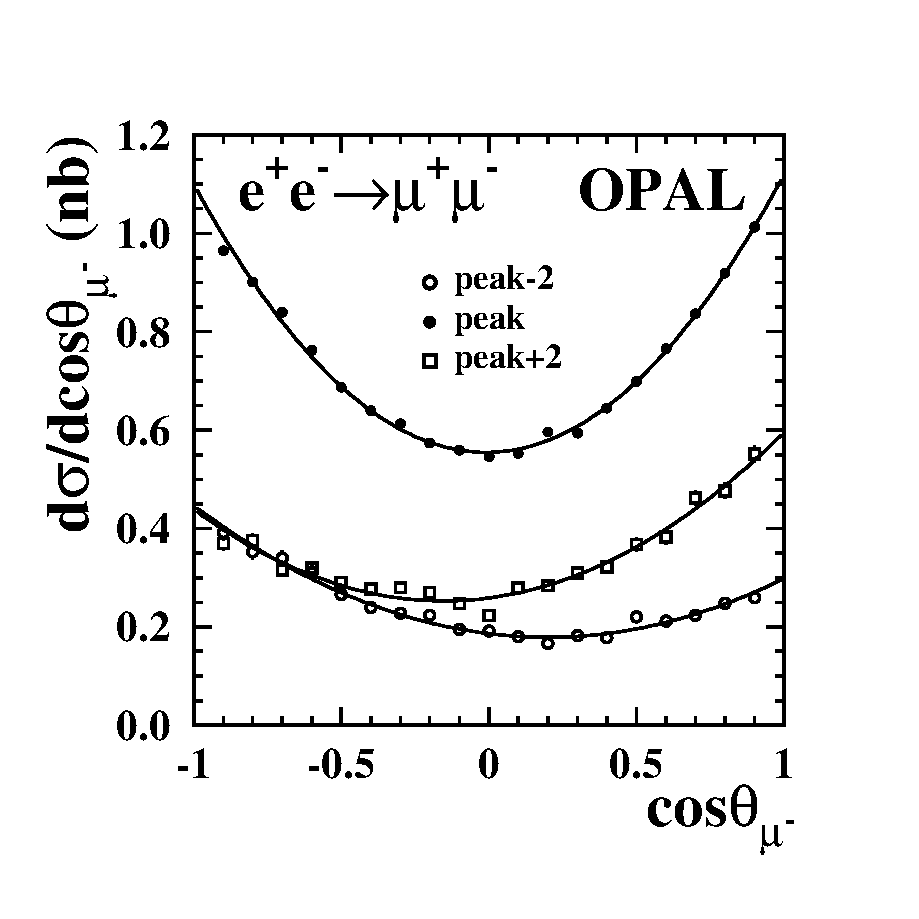
\includegraphics[scale=0.5]{Images/SM-test-5.eps}
  \caption[Asimetría forward-backward]{La asimetría \textit{forward-backward} a pesar de ser pequeña es claramente un indicador de que el bosón Z acopla diferente con los fermiones de mano derecha e izquierda. $A_{\rm FB}=0$ para procesos mediados puramente por QED  \cite{opal2001precise}.}
 \label{SMt5}
\end{figure}



\section[\hspace{-0.19in} Física del Higgs]{Física del Higgs}

%\color{red}
%(to be completed): read Maggiore.
%\color{black}


Descubierto en 2012 por las colaboraciones ATLAS \cite{ATLAS:2012yve} y CMS \cite{CMS:2012qbp}, el bosón de Higgs es la pieza final del modelo estándar. Esta partícula es especial en el sentido de que es la única partícula fundamental con spin cero que conocemos. Sus decaimientos han sido estudiados ampliamente; sin embargo, poco se sabe de su acople trilinear y además hay indicios de que podría haber otros escalares neutros más ligeros \cite{CMS:2018cyk,CMS:2023yay,CMS:2024yhz} o más pesados \cite{Kundu:2024sip} que estarian al alcance de próximos experimentos.

Se conocerá más sobre el Higgs, por ejemplo, en futuros colisionadores de muones ya que tienen la ventaja de ser de precisión como los colisionadores de $e^+e^-$ y llegarían a altas energías comparables a la de los del gran colisionador hadrónico \footnote{Un colisionador de muones a energía de centro de masa de 10 TeV es comparable con el LHC a 100 TeV \url{https://home.cern/science/accelerators/muon-collider}.}.


\section[\hspace{-0.2in} Conclusiones]{Conclusiones}

El modelo estándar ha probado ser un gran logro de la ciencia moderna. En este capítulo, hemos visto como ha superado varios tests en colisionadores, lo cual justifica su nombre. Sin embargo, el no incluir a, por ejemplo, la interacción gravitacional, es una señal de que debemos ir más allá de este modelo.
%\color{red}
%conclusiones de este capítulo: El ME es genial, funciona muy bien, pero todavia necesitamos más experimentos. Futuros experimentos como el colisionador de muones podrán testar triple vertex (limites superiores aún son muy débiles )
%\color{black}
















\chapter[\hspace{-0.15in}.  Más allá del Modelo Estándar]{II. Más allá del Modelo Estándar}
% ==============
% Materia oscura
% ==============

Habiendo visto como el modelo estándar concuerda excelentemente con los resultados de experimentos terrestres a altas energías, veamos ahora algunas evidencias cosmológicas que apuntan a que debemos pensar en ir más allá de este modelo.

%\color{red}
%objetivo de este capítulo
%\color{black}


\section[\hspace{-0.14in}Materia oscura]{Materia oscura}

Históricamente la investigación en materia oscura comenzó en 1933 cuando el astrónomo suizo Fritz Zwicky observó que `faltaba materia' en el cúmulo de galaxias Coma \cite{zwicky}\footnote{La versión en inglés puede encontrarse aqui \cite{zwicky2009republication}.}. Posteriormente otros investigadores descubrieron que esta materia faltante, denominada \textit{materia oscura} por Zwicky, podria explicar observaciones cosmológicas como curvas de rotación planas en galaxias espirales \cite{Vera,rubin1978extended}, el efecto de lentes gravitacionales de cúmulos de galaxias y el \textit{bullet cluster} \cite{clowe2006direct}, entre otras \footnote{Las teorías de la dinámica newtoniana modificada (MOND en inglés) son alternativas a la hipótesis de la materia oscura como partícula, pero no serán discutidas en este trabajo.}. A continuación veremos brevemente cómo aparece la materia oscura en diferentes escenarios cosmológicos y porqué se piensa que su naturaleza no es de origen bariónico.


% ----------------------------
% Evidencias de materia oscura
% ----------------------------
\subsection[\hspace{-0.4in}) Evidencias]{Evidencias}




\begin{itemize}
% -----------------------------------------------------
% Evidencias de materia oscura: Cúmulos de galaxias
% -----------------------------------------------------

\item[1] \textbf{Dispersión de velocidades en cúmulos de galaxias}: En su artículo de 1933 `El corrimiento al rojo de las nebulosas extragalácticas', Fritz Zwicky estudió el cúmulo de galaxias Coma y demostró, mediante el teorema del virial, que la densidad de la materia oscura es mucho mayor que la de la materia luminosa. Suponiendo que el cúmulo de Coma es un sistema mecánicamente estacionario, el teorema del virial nos dice que la energia cinética media $\left<\mathcal{E}_k\right>$ y potencial media $\left<\mathcal{E}_p\right>$ están relacionadas por
\begin{equation}
    \left<\mathcal{E}_k\right> = - \frac{1}{2}\left<\mathcal{E}_p\right>.
    \label{virial}
\end{equation}
Para fines de estimación, supongamos una distribución uniforme de masa ($\rho$ = constante) en el cúmulo de Coma. De esta manera, si $M$ y $R$ representan su masa lumínica y radio, respectivamente, entonces su energía gravitacional $U$ es
\begin{equation}
    U=-\int_0^M G\frac{\, m(r)}{r} dm = -\frac{3}{5}\frac{GM^2}{R}.      
\end{equation}
De este resultado y la ecuación (\ref{virial}), obtenemos
\begin{equation}
    \frac{1}{2} M \left< v^2 \right> =\left<\mathcal{E}_k\right> = - \frac{1}{2}\left<\mathcal{E}_p \right> =- \frac{1}{2} U  = \frac{3}{10}\frac{GM^2}{R},
    \label{vM}
\end{equation}
lo que resulta en
\begin{equation}
    \left< v^2 \right>^{1/2} \approx \rm 80 \, km/s.
\end{equation}
Con este resultado, la dispersión de velocidades $\sigma = \left[\left< v^2 \right> - \left< v \right>^2 \right]^{1/2}\leq \left< v^2 \right>^{1/2}$ en el cúmulo de Coma está muy debajo de lo observado, \textit{i.e.} 1500 a 2000 km/s \cite{zwicky, zwicky2009republication}. Este problema hizo que Zwicky concluyera que, como $\left< v^2\right>^{1/2} \propto \sqrt{M}$ de la ecuación (\ref{vM}), el cúmulo necesitaba que su masa fuera al menos \textit{400 veces mayor} que la masa de su materia luminosa. A esta materia no observada él la llamó \textit{materia oscura}.

% -------------------------------------------------------
% Evidencias de materia oscura: Curvas de rotación planas
% -------------------------------------------------------

\item[2] \textbf{Curvas de rotación planas}: En una galaxia esférica\footnote{Hay galaxias esféricas como algunas galaxias enanas, pero hay otras que no lo son como las enanas irregulares, las galaxias elípticas y las espirales.}, de la mecánica newtoniana se espera la siguiente relación entre la velocidad de rotación $v$ y la distancia a su centro $r$,
\begin{equation}
v \propto \bigg\lbrace
\begin{array}{cc} 
r,&~\text{dentro de la galaxia} \\ 
r^{-1/2},~ &\text{fuera de la galaxia} 
\end{array}.
\label{vr-relation}
\end{equation}
Una curva de rotación es plana cuando $v$ no cae como $r^{-1/2}$ en sus afueras sino se mantiene constante. En 1970, Vera Rubin y Kent Ford mostraron la primera evidencia de curvas de rotación planas en las galaxias \cite{Vera}. En la figura \ref{rotationcurve} podemos ver la curva de rotación plana de la galaxia espiral NGC 3198.

Los modelos que intentan resolver esta discrepancia entre teoria y observación generalmente toman en consideración dos distribuciones distintas de materia. Por ejemplo, para NGC 3198 se podria usar una distribución de materia luminosa de tipo disco y un halo (esférico) de materia oscura \cite{van2004distribution}. Como resultado, los modelos de dos componentes generalmente obtienen buenos ajustes (ver Fig.\ref{rotationcurve}).

\begin{figure}[h!]
\centering
  \includegraphics[width=.8\linewidth]{Images/NGC3198.png}
  \caption[Curva de rotación de la galaxia espiral NGC 3198]{Curva de rotación de la galaxia espiral NGC 3198 \cite{van2004distribution}. La curva de rotación de la galaxia espiral NGC 3198 no puede modelarse con éxito únicamente mediante un disco de materia bariónica. Se debe agregar un halo de materia invisible para que coincida con las observaciones.}
  \label{rotationcurve}
\end{figure}


% -------------------------------------------------
% Evidencias de materia oscura: Relaciones masa-luz
% -------------------------------------------------
    
    \item[3] \textbf{Relaciones masa-luz}: La forma del universo siempre ha sido de gran interés para la humanidad. Es posible saber si es abierto, cerrado o plano determinando la relación entre su densidad de masa $\rho$ y la densidad crítica $\Omega=\rho/\rho_c$. Un universo plano $\Omega = 1$ es consistente con las observaciones \cite{Workman:2022ynf}. 
    
    Si consideramos que la masa del universo es principalmente la suma de las masas de sus partes visibles, {\it es decir} las galaxias, entonces al encontrar la relación masa-luz de una sola galaxia (suponiendo que esto sea igual para todo el universo) y multiplicarla por la luminosidad del universo debería darnos la masa del universo y, en consecuencia, $\Omega$.
    
    La luminosidad de los objetos astronómicos en el universo revela una densidad de luminosidad total de $\rho_L=2.0\pm0.7 \times 10^{8}hL_{\odot}Mpc^{-3}$ \cite{efstathiou1988analysis}. Como la densidad crítica está dada por $\rho_c=3H_0^2/8\pi G=2.775 37(13)\times 10^{11}\Omega h^2 M_{\odot}Mpc^{-3}$ \cite{patrignani2016review}, para un universo plano la relación masa-luz es \cite{peacock1999cosmological}
    \begin{equation}
    \left( \frac{M}{L} \right)_{\rm plano} = 1390h \times \left( \frac{M_\odot}{L_\odot} \right),
    \label{criticalmasstolight}
    \end{equation}
    donde $M_\odot$ y $L_\odot$ son la masa y luminosidad del sol, respectivamente, y $h=0.674$ \cite{Workman:2022ynf}.
    
   Para el cúmulo de galaxias Coma, $M/L\simeq300h$ en unidades solares \cite{zwicky,zwicky2009republication}. Dado que este valor está lejos del resultado obtenido en la ecuación (\ref{criticalmasstolight}), se necesitan más objetos masivos de baja luminosidad para obtener nuestro universo plano observado.



% ----------------------------------------------------
% Evidencias de materia oscura: Lentes gravitacionales
% ----------------------------------------------------
    \item[4] \textbf{Lentes gravitacionales}: Los cúmulos de galaxias se pueden utilizar como telescopios porque la gravedad puede `doblar' la luz. Estos cúmulos de galaxias desviarán la luz proveniente de, digamos, una sola galaxia o un grupo de ellas (ver Fig.\ref{gravlens}), y la medida de la deflexión nos dará la masa del cúmulo. Los resultados de la lente parecen coincidir con la relación masa-luz $M/L \simeq 300h$ obtenida del estudio del cúmulo de Coma \cite{zwicky,zwicky2009republication}, lo que refuerza la afirmación de que falta masa en los cúmulos de galaxias.

\begin{figure}[h]
  \centering
  \includegraphics[height=.6\linewidth]{Images/ABELL2218.png}
  \caption[Cúmulo de galaxias Abell 2218]{Cúmulo de galaxias Abell 2218 \cite{fruchterNASA}. La luz procedente de objetos luminosos situados detrás del cúmulo de galaxias Abell 2218 es desviada por éste creando arcos tenues.}
  \label{gravlens}
\end{figure}


% ------------------------------------------------------------------
% Evidencias de materia oscura: El fondo cósmico de microondas (CMB)
% ------------------------------------------------------------------
\item[5] \textbf{El fondo cósmico de microondas (CMB)}: Las mediciones de la temperatura del fondo cósmico de microondas hecho por el satétile de Planck\footnote{\textit{Planck} es la misión de la Agencia Espacial Europea para mapear el cielo midiendo la temperatura y las anisotropías de polarización de la radiación cósmica de microondas.} dio como resultado las densidades relativas $\Omega_b h^2=0.02205(28)$ para los bariones y $\Omega_{DM} h^2=0.1199(27)$ para la materia oscura fria. Ambos resultados son inferidos en el contexto del modelo cosmológico estándar $\Lambda$CDM \cite{ade2014planck} .
A partir de estos resultados, se puede ver que no sólo la materia barionica no es el componente dominante en la densidad de energía del universo, sino que además la mayor parte esta última es de composición desconocida.


\begin{figure}[h]
\centering
  \includegraphics[width=.85\linewidth]{Images/CMB.png}
\caption[Fondo cósmico de microondas]{Fondo cósmico de microondas \cite{CMBWMAP}. La imagen detallada del universo primitivo revela fluctuaciones de temperatura de 13,77 mil millones de años, que fueron las semillas que crearon las galaxias.}
  \label{CMB}
\end{figure}




% ----------------------------------------------------------------------
% Evidencias de materia oscura: La estructura a gran escala del Universo
% ----------------------------------------------------------------------
    \item[6] \textbf{La estructura a gran escala del Universo}: Como el parámetro de densidad bariónica $\Omega_b$ es muy pequeño en comparación con los otros `ingredientes' del universo, habría requerido grandes fluctuaciones en el universo primordial en la densidad bariónica para formar el número actual de galaxias observadas \cite{peacock1999cosmological}. Estas grandes fluctuaciones también significarían grandes anisotropías en el fondo cósmico de microondas. En consecuencia, la formación de galaxias en un medio puramente bariónico queda totalmente descartada por la observación de pequeñas anisotropías en el CMB (Fig.\ref{CMB}). 
    
    Por otra parte, la materia oscura fria puede formar pozos gravitacionales ideales para la formación de galaxias. Esto se debe a que ella puede desacoplarse del plasma primordial mucho antes que los bariones, lo que daria tiempo al crecimiento de inhomogeneidades y el subsecuente colapso gravitacional necesario \cite{Kolb:1990vq}. 
    
% ------------------------------------------------
% Evidencias de materia oscura: El cúmulo de balas
% ------------------------------------------------
\item[7] \textbf{El cúmulo de balas}: En los trabajos más recientes sobre cosmología observacional destacan la presencia de materia oscura en colisiones de cúmulos de galaxias. En la figura \ref{bulletcluster} vemos la colisión de dos cúmulos de galaxias fusionándose en un cúmulo doble (cúmulo de galaxias 1E 0657-56), que se conoce como {\it bullet cluster} por el gas caliente en forma de bala que se asemeja a una bala supersónica produciendo ondas de choque.

Los principales ingredientes de estas colisiones son galaxias, nubes de gas caliente y materia oscura. Como las galaxias están muy distantes unas de las otras, no participan mucho en las colisiones. Sin embargo, los gases calientes chocan, produciendo un frente de choque (Fig.\ref{bulletcluster}) y, lo más importante, separándose de la materia oscura. ¿Cómo podemos saber esto? Como se puede ver en la figura \ref{DMgravpot}, el mapa del potencial gravitacional indica claramente la presencia de dos objetos \textit{invisibles} masivos que dominan en términos de masa en este sistema y se encuentran lejos del componente lumínico dominante (el gas ionizado).



\begin{figure}[h]
\centering
  \includegraphics[width=.75\linewidth]{Images/bulletcluster.jpg}
  \caption[Cúmulo doble de galaxias 1E 0657-56: Bullet cluster]{Cúmulo doble de galaxias 1E 0657-56: el \textit{bullet cluster} \cite{clowe2006direct}. En la colisión de dos cúmulos de galaxias, el gas ionizado caliente del cúmulo más pequeño adquiere la forma de una bala, produciendo así un frente de choque en forma de arco.}
  \label{bulletcluster}
\end{figure}


\begin{figure}[h]
\centering
  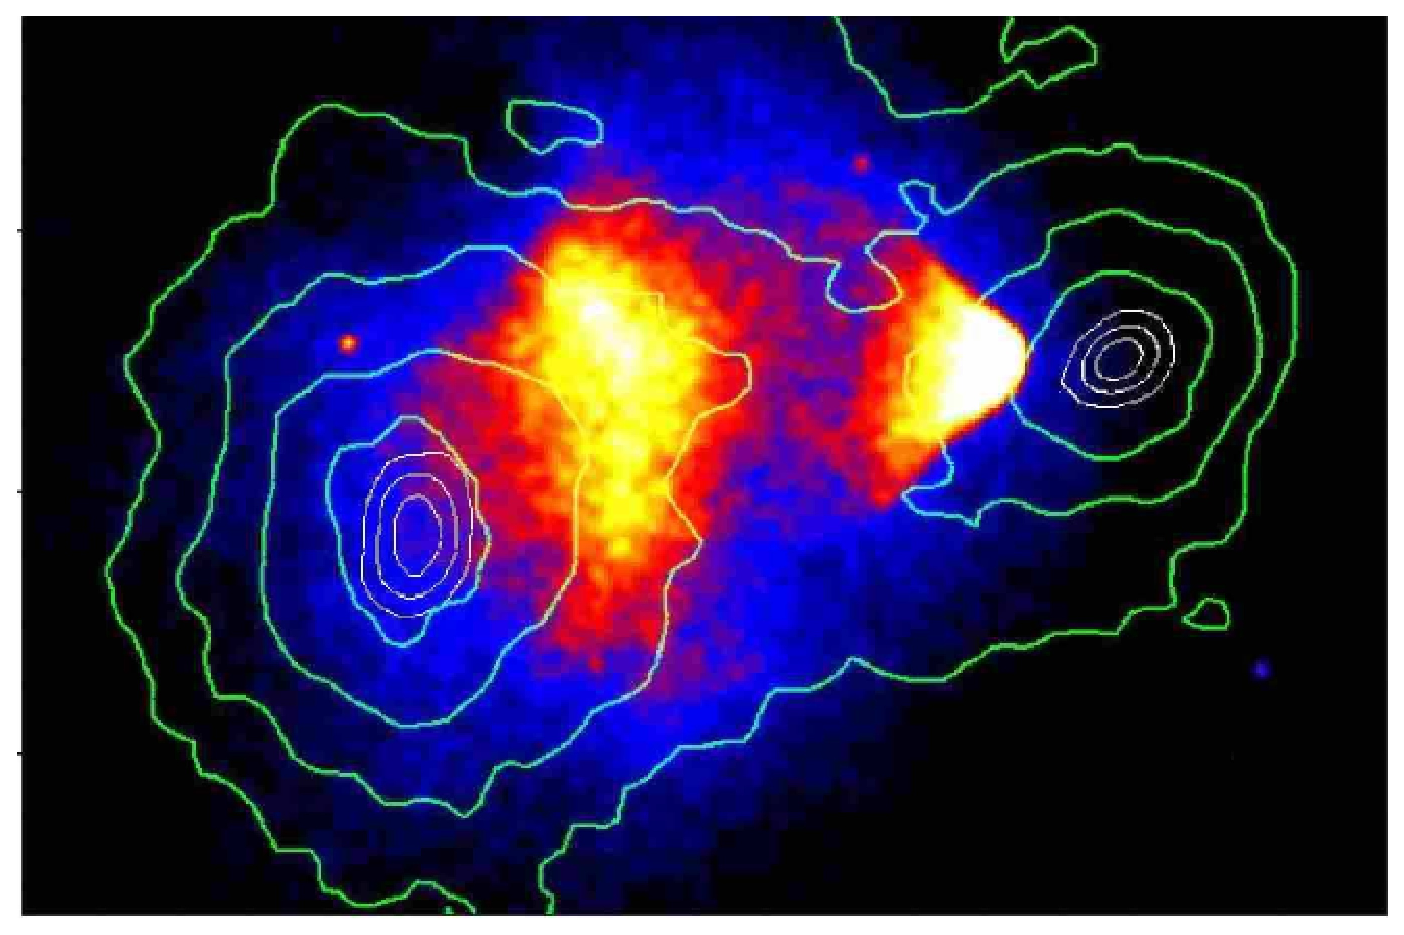
\includegraphics[width=.9\linewidth]{Images/BCgravpot.eps}
  \caption[El potencial gravitacional en el Bullet cluster]{Mapa del potencial gravitacional en la colisión de dos cúmulos de galaxias \cite{clowe2006direct}. La colisión de dos grandes cúmulos no podría exhibir esta forma de potencial gravitacional si no fuera por la materia oscura que es dominante y se ha separado del gas y las estrellas.}
  \label{DMgravpot}
\end{figure}

% -----------------------------------------
% Evidencias de materia oscura: Microlentes
% -----------------------------------------
\newpage
\item[8] \textbf{Microlentes}: Este fenómeno astronómico se basa en el efecto de lente gravitacional y utiliza el movimiento relativo entre la fuente y la lente para `aclarar' temporalmente la señal combinada. Esto significa que es posible encontrar objetos que emiten poca o ninguna luz monitoreando las curvas de luz provenientes de la fuente, las cuales son desviadas y distorsionadas.

En la figura \ref{Amplification-LigthCurve} vemos como aparecen dos picos (amplificación $A>1$) momentáneos en las bandas azul y roja en la curva de luz de una estrella en la Gran Nube de Magallanes. La curva teórica proveniente de un modelo de halo oscuro en nuestra galaxia \cite{paczynski1986gravitational} hace un fit excelente a las amplificaciones en las dos bandas \cite{alcock1993possible}. Esta no es una prueba definitiva de la presencia de materia oscura pero sí de que existe un halo oscuro masivo alrededor de la Vía Láctea.
\end{itemize}


\begin{figure}[h]
\centering
  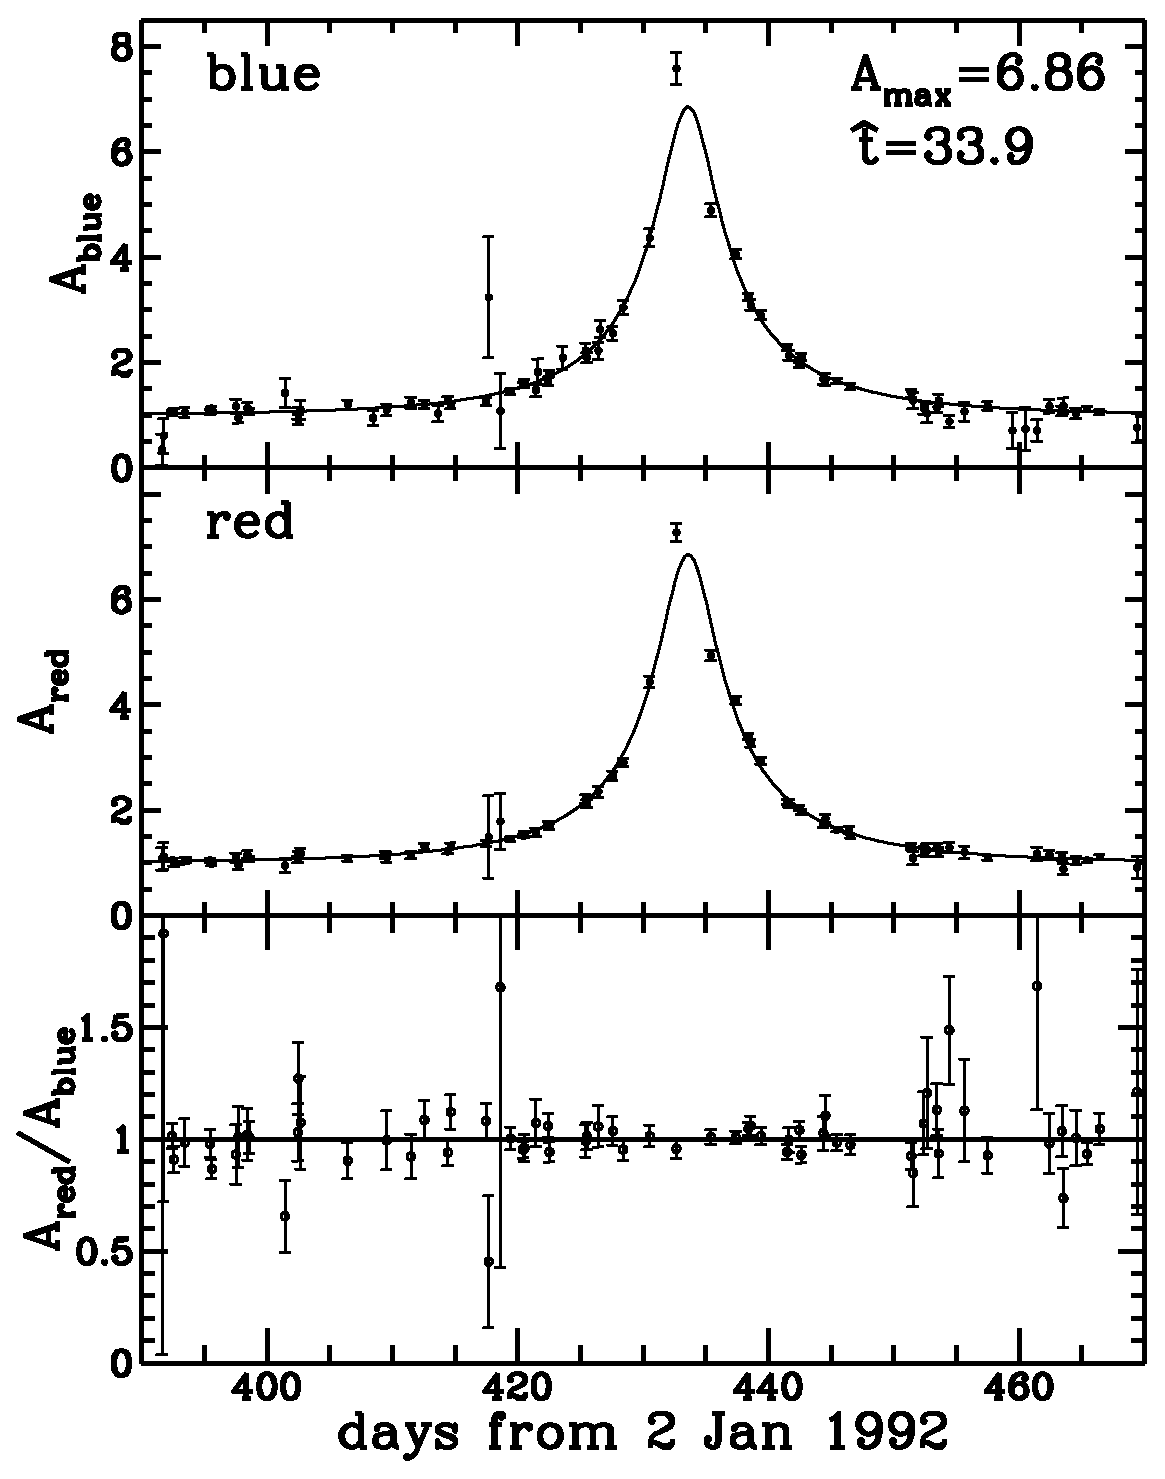
\includegraphics[height=0.8\linewidth]{Images/fluxes.eps}
  \caption[Microlentes: Curva de luz de una estrella en la nube de Magallanes]{Curva de luz de una estrella en la nube de Magallanes \cite{alcock1993possible}. La luz de fuente, en este caso una estrella, es amplificada por un objeto que no ha podido ser observado directamente. Este evento favorece la hipótesis de un halo oscuro alrededor de nuestra galaxia.}
\label{Amplification-LigthCurve}
\end{figure}



\newpage
\subsection[\hspace{-0.4in}) Partícula masiva que interactúa débilmente (WIMP)]{Partícula masiva que interactúa débilmente (WIMP)}

Como acabamos de ver, exiten fuertes evidencias de la presencia dominante, en términos cosmológicos, de (por lo menos) un tipo de materia desconocida la cual se le denomina materia oscura. A pesar de no saber con exactitud de qué está formada esta materia oscura, se puede deducir sus propiedades de manera general en el modelo cosmológico estándar \cite{Arcadi:2024ukq}. A continuación listamos  estas propiedades.

\begin{itemize}
\item[1.] \textbf{Estabilidad}. Las observaciones locales y a gran escala muestran que la materia oscura representa aproximadamente el 85$\%$ del total de materia. Como el tiempo de vida del universo es aproximadamente 13.8 Gyr, esta materia oscura debe ser estable o, caso contrário, tener un tiempo de vida média mucho mayor que la edad del universo.
\item[2.] \textbf{Interacciones débiles}. Hasta el momento no se ha observado ninguna señal de interacciones de materia oscura con la materia del modelo estándar en experimentos de detección directa como LUX, PandaX-II o XENONnT. Sumándole el hecho de que la materia oscura debe tener carga eléctrica nula para explicar, por ejemplo, las curvas de rotación de las galáxias, se puede concluir que las interacciones de la materia oscura con la materia ordinaria debe ser muy débil. 
%Experimentos de detección directa han descartado secciones de choque de WIMPs con nucleones llegando hasta $10^{-46}$ cm$^2$ (LUX y PandaX-II), $10^{-47}$ cm$^2$ XENONnT y se proyectan sentividades de hasta $10^{-49}$ cm$^2$ DARWIN.
\item[3.] \textbf{Mecanismo de producción}. Observaciones del fondo cósmico de microondas revelan que la materia oscura estaba presente en aquella época temprana del universo. Esto quiere decir que la materia oscura debe haber sido producida por algún mecanismo en el universo temprano antes de la formación del CMB, por ejemplo, freeze-out (ver apéndice). La densidad actual de materia oscura debe ser explicada por este mecanismo.
\item[4.] \textbf{Adecuado para la formación de estructuras}. La materia oscura es uno de los principales actores en la formación de galaxias ya que provee el pozo de potencial para capturar la materia ordinaria. Para que esto suceda, la materia oscura debe ser no relativista y muy abundante en la época de igualdad materia-radiación. 
\item[5.] \textbf{Autointeracciones}. Como vimos en el item 2, las interacciones de la materia oscura con la materia ordiaria debe ser muy débil. Sin embargo, esto no descarta la posibilidad de que la materia oscura pueda interactuar consigo misma o con partículas de un sector oscuro. En particular, para explicar las observaciones del cúmulo de balas (bullet cluster) se debe tener $\sigma/m <$ 1 cm$^2$/g \cite{Markevitch:2003at}.
\end{itemize}

Una clase popular de candidatos a materia oscura son partículas masivas que interactúan débilmente (WIMP)\footnote{Weakly Interactive Massive Particle.}. Estas partículas generalmente tienen una sección de choque `correcta' $\left< \sigma v\right> \sim 3 \times 10^{-26}$ cm$^3$/s para masas de GeV$-$TeV, lo que las hace fuertes candidatos \cite{profumo2017introduction}. Los WIMPs obtienen su densidad de relíquia del proceso de desacoplamiento del plasma primordial en las primeras etapas de la historia del universo lo que les da una densidad comóvil constante la cual se mantiene hasta el presente.

% --------------------------------------------------------------------------------------------------------
\section[\hspace{-0.14in}Detección directa e indirecta de materia oscura]{Detección directa e indirecta de materia oscura}
% -------------------------------------------------------------------------------------------------------- 

La búsqueda de materia oscura se da a través de experimentos de detección directa, detección indirecta y producción en colosionadores. Si bien la materia oscura interactua muy poco con las partículas del modelo estándar, procesos a nivel de loop podrían dar señales de ella. En la figura \ref{fig_DMsearches} se muestra como estos procesos provenientes de nueva física podrían producir partículas de materia oscura en experimentos con colisionadores como el LHC y como puede darse la detección directa e indirecta de materia oscura. Si bien estas búsquedas son complementarias, cada una de ellas es un tema muy amplio y por eso dejaremos este estudio para futuros trabajos. Sin embargo, comentaremos un poco sobre estas búsquedas de materia oscura.

%en esta tesis nos enfocaremos en poner límites a un candidato a materia oscura proveniente del $3-3-1$ Económico por medio de detección indirecta. %ya que detección directa tiene el background irreducible de neutrinos (ver Strumia's review) Queiroz:2016awc

\begin{figure}[h]
\centering
\includegraphics[scale=0.45]{Images/DM-searches.pdf}
\caption[Interacciones de la materia oscura]{Diferentes tipos de interacción de la materia oscura ($\chi$) con partículas del modelo estándar (ME). Nótese que los procesos horizontales determinan la densidad de materia oscura proveniente del freeze-out térmico ya que este proceso cambia el número de partículas de materia oscura.}
\label{fig_DMsearches}
\end{figure}


\subsection[\hspace{-0.4in}) Detección directa]{Detección directa}
La detección directa de materia oscura es un enfoque experimental que busca identificar interacciones entre partículas de materia oscura y materia ordinaria. Este tipo de detección se basa en la hipótesis de que las partículas de materia oscura, como los WIMPs, podrían interactuar débilmente con núcleos atómicos a través de colisiones elásticas, causando un retroceso nuclear detectable. Para ello, los experimentos utilizan detectores extremadamente sensibles, ubicados en laboratorios subterráneos para minimizar el ruido de fondo proveniente de rayos cósmicos y otras fuentes de radiación \cite{profumo2017introduction}. 

Los detectores suelen emplear tecnologías avanzadas, como cristales de germanio, xenón líquido o argón líquido, que pueden registrar pequeñas cantidades de energía liberadas en los retrocesos nucleares. La señal de materia oscura esperada es extremadamente débil\footnote{La energía depositada por las partículas de materia oscura en los detectores es del orden de eV$-$keV \cite{Cirelli:2024ssz}.} , por lo que estos experimentos están diseñados para discriminar entre posibles eventos de materia oscura y señales de fondo, como radiación gamma o neutrones. Además, las técnicas de análisis buscan patrones característicos, como una modulación anual debida al movimiento relativo de la Tierra a través del halo de materia oscura.

\begin{figure}[h]
\centering
\includegraphics[scale=0.55]{Images/WIMP-DD.pdf}
\caption[\hspace{0.05in}Límites en la sección de choque de los WIMPs]{Límites en la sección de choque (independiente del spin) de un WIMP con nucleones \cite{Cooley:2014aya}.}
\label{WIMPDD}
\end{figure}

Aunque hasta ahora no se ha detectado directamente materia oscura, estos experimentos han impuesto límites estrictos sobre la probabilidad de interacción (sección de choque) y en función de las masas de las partículas candidatas a materia oscura, ver figura \ref{WIMPDD}. 

\subsection[\hspace{-0.4in}) Perfiles de materia oscura]{Perfiles de materia oscura}
%\subsection{Fermi-LAT}
La materia oscura en las galáxias se encuentra distribuida en toda su extensión y por este motivo estas se modelan típicamente usando un halo de materia oscura. La forma de este halo depende del tipo de galáxia. Perfiles comúnmente usados en la literatura son Navarro-Frenk-White (NFW) \cite{Navarro:1995iw} y Einasto \cite{einasto1965kinematics}, los cuales provienen de simulaciones de N-cuerpos de alta resolución, ver figura \ref{profiles}.

\begin{figure}[h]
\centering
\includegraphics[scale=0.5]{Images/profiles.pdf}
\caption[\hspace{0.1in}Perfiles de densidad de materia oscura]{Perfiles de densidad de materia oscura: NFW, Einasto y NFW cored (NFWc) \cite{Angel:2023rdd}.}
\label{profiles}
\end{figure}

NFW es el perfil de materia oscura más popular ya que se basa en materia oscura fria que `no colisiona'\footnote{Collisionless cold dark matter.}, esto es interacciones puramente gravitacionales. Este perfil consigue reproducir bien las curvas de rotación de varias galáxias, sin embargo, en el centro de ellas aparece un problema: la densidad central de NFW es mayor de la requerida para explicar la parte central de las curvas de rotación de las galáxias. Ante esto, otras opciones aparecen, tales como NFWc\footnote{Contracted NFW.} y Einasto. La primera viene de generalizar NFW usando
\begin{equation}
\rho (r) = \frac{\rho_0}{(r/r_s)^\gamma (1+r/r_s)^{3-\gamma}},
\end{equation}
donde $\gamma$ es un parámetro libre: $\gamma =1$  para NFW y $\gamma = 1.3$ para NFWc. Para Einasto tenemos
\begin{equation}
\rho (r) = \rho_0 \exp \left\{ - \frac{2}{\alpha} \left[ \left( \frac{r}{r_0}\right)^\alpha -1 \right] \right\}.
\end{equation} 

\subsection[\hspace{-0.4in}) Detección indirecta]{Detección indirecta}
La materia oscura, a pesar de ser estable en escalas cosmológicas, podría dar señales de su presencia al aniquilarse en regiones de alta concentración como el centro galáctico o galáxias enanas y producir partículas del modelo estándar que podamos detectar en la Tierra. El programa de detección indirecta de materia oscura se basa en identificar fotones, neutrinos y rayos cósmicos provenientes de estas aniquilaciones\footnote{También se buscan los productos de decaimientos de materia oscura, pero no abordaremos ese tema en este trabajo.}. Los fotones y los neutrinos son de particular interés porque viajan en línea recta (a diferencia de los rayos cósmicos que son cargados eléctricamente) y por eso se puede saber de dónde vienen. Los neutrinos, a pesar de ser muy numerosos, son difíciles de detectar ya que estos tienen secciones de choque muy pequeñas. Por otro lado, los fotones tienen secciones de choque mayores y pueden ser producidos con un espectro de energía contínuo o discreto (línea) proveniente de aniquilaciones de materia oscura ($\mathcal{DM}\, \mathcal{DM} \to \gamma \gamma$) donde la energía de los fotones es $E_\gamma = m_\mathcal{DM}$. En la figura \ref{fig:g_Servant} se muestra como ejemplo el flujo de fotones para una materia oscura de 300 GeV \cite{Jackson:2013pjq}.
\begin{figure}[h]
\centering
\includegraphics[scale=1]{Images/fig_Servant.pdf}
\caption[Espectro de rayos gamma (línea)]{Espectro de rayos gamma para un modelo donde la materia oscura tiene 300 GeV de masa. El pico que se distingue del espectro contínuo viene de la producción directa $\mathcal{DM}\, \mathcal{DM} \to \gamma \gamma$ donde $E_\gamma = m_\mathcal{DM} =300$ GeV. Imagen adaptada de \cite{Jackson:2013pjq}.}
\label{fig:g_Servant}
\end{figure}

La forma de calcular este flujo de fotones\footnote{Flujo diferencial de una dirección angular $d\Omega$.} llegando a la Tierra es (vea, por ejemplo, \cite{Cirelli:2010xx,Queiroz:2016awc,Slatyer:2021qgc})
\begin{equation}
\frac{d\Phi_{\gamma}}{d\Omega \, dE} = \frac{1}{2} \frac{r_\odot}{4\pi} \left( \frac{\rho_\odot}{m_\mathcal{DM}} \right)^2 J \sum_f \left< \sigma \, v \right>_f \frac{dN_\gamma^f}{dE},
\end{equation}
donde $r_\odot=8.33$ kpc es la posición del sol respecto al centro galáctico, $\rho_\odot=0.3$ GeV/cm$^3$ es la densidad de la materia oscura cerca al sol \cite{gillessen2009monitoring}, $m_\mathcal{DM}$ es la masa de la materia oscura, $dN_\gamma^f/dE$ es el espectro de energia de los fotones producidos por aquinilación, el factor $J$ está dado por
\begin{equation}
J = \int_{\rm l.o.s.} \frac{ds}{r_\odot} \left( \frac{\rho (r(s,\theta))}{\rho_\odot} \right)^2,
\end{equation}
y $\left< \sigma \, v \right>_f$ es la sección de choque térmicamente promediada en el canal con estado final $f$. Esta ecuación es válida para partículas de materia oscura que sean auto-conjugadas, por ejemplo fermiones de Majorana. Cuando este no sea el caso, debe promediarse sobre partículas y antipartículas, entonces aparece un factor multiplicativo extra, $1/2$.




%\subsection{H.E.S.S.}

%El Sistema Estereoscópico de Alta Energía\footnote{High Energy Stereoscopic System.} (H.E.S.S.) es un arreglo de telescópios atmosféricos Cherenkov para la investigación de los rayos gamma cósmicos en el rango de energía de los fotones de GeV$-$TeV.

%Estos rayos gamma podrían provenir de la aniquilación de materia oscura en regiones altamente densas como el centro de la galáxia. Se espera que de las aniquilaciones de materia oscura en quarks, leptones pesados o bosones vectoriales, junto con una emisión secundaria proveniente de scattering de Compton inverso asi como de bremsstrahlung de electrones producidos en la cadena de decaimientos, produzca un contínuo de rayos gamma. El background de fotones provenientes de otros procesos astrofísicos hace que la distinción de esta señal algo no trivial \cite{HESS:2018cbt}.

%Por ortra parte, los decaimientos en líneas de rayos gamma\footnote{$\gamma-ray$ lines.} provenientes de la aniquilación de materia oscura en `reposo' ($v \sim 10^{-3}c$) en $\gamma+X$ donde $X=\gamma, Z, h$ u otras partículas del sector oscuro, producen una línea espectral angosta con energía $E_\gamma =m_{\rm DM}(1-m_X^2/4m^2_{\rm DM})$, la cual está limitada por la resolución del detector. Para H.E.S.S. la resolución de energía es $10\%$. Cuando la materia oscura se aniquila en partículas cargadas, existen rayos gamma adicionales provenientes de radiación en estado final\footnote{Final state radiation (FSR).} y bremsstrahlung interno.

%Como vimos anteriormente, la distribución de materia oscura en la galáxia es muy importante para el cálculo del flujo de rayos gamma. La colaboración H.E.S.S. trabajó con dos perfiles: NFW y Einasto. Los resultados de 10 años de observaciones de H.E.S.S. se muestran en la figura \ref{HESS_sigmav}. Se puede ver que llegan a poner límites superiores a $\left< \sigma \, v \right>$ hasta $10^{-27}$cm$^3$/s para el perfil NFW y aún menores abajo para Einasto. Como comparación se muestran también resultados de otras colaboraciones como la de Fermi-LAT que es dominante en una región donde no llega H.E.S.S.


\begin{figure}[h!]
\centering
\includegraphics[scale=0.5]{Images/HESS.pdf}
\caption[Limites para $\left< \sigma \, v \right>$ provenientes de H.E.S.S.]{Limite superior para $\left< \sigma \, v \right>$ para el proceso de aniquilación de materia oscura en rayos gammas proveniente de 10 años de observaciones del halo galáctico interno. Imagen adaptada  de \cite{HESS:2018cbt}.}
\label{HESS_sigmav}
\end{figure}

\newpage
% ----------------------------------------------------------------------------------- 
\section[\hspace{-0.14in}Modelo $\nu_R$-331]{Modelo $\nu_R$-331}
% -----------------------------------------------------------------------------------

%\color{red}
%Leer paper de Vicente: resumen 3-3-1
%\color{black}

Los modelos $3-3-1$ surgen al reemplazar el grupo de gauge del modelo estándar G$_{\rm SM} \equiv SU(3)_C \times SU(2)_L \times U(1)_Y$ por G$_{\rm 3-3-1} \equiv SU(3)_C \times SU(3)_L \times U(1)_X$, donde $C$ y $L$ son color y quiralidad izquierda, respectivamente, y $X$ representa una nueva carga diferente de la hipercarga $Y$ del modelo estándar.

Aqui, el operador de carga eléctrica se puede escribir como \cite{Pleitez:2021abk},
\begin{equation}
Q_{\beta}(X) = a T_3 + \beta T_8 + X \mathds{1}_{3\times 3},
\end{equation}
donde $T_3$ y $T_8$ son las matrices diagonales de Gell-Mann, y $\mathds{1}_{3\times 3}$ es la matriz identidad. 

Para fines prácticos, en este trabajo seguiremos \cite{sanchez2019vacuum} tomando\footnote{Otros valores para $\beta$ son $\sqrt{3},-\sqrt{3}$ y $1/\sqrt{3}$.} $a=1$, $\beta = -1/\sqrt{3}$ y trabajando con el sector escalar más simple para modelos sin cargas eléctricas exóticas \cite{Foot:1994ym,Ponce:2001jn}. A este modelo se le conoce en la literatura como modelo $\nu_R-331$ \cite{Singer:1980sw}.

En este modelo, por ejemplo, los neutrinos de mano derecha $N_a \ (a=1,2,3)$ se encuentran juntos con los leptones del modelo estándar en el mismo multiplete de $SU(3)_L$,
\begin{eqnarray}
\text{Leptones} : \text{L}_{aL} = \left( \begin{array}{c}
\nu_a \\ \ell_a  \\ N_a^c
\end{array} \right)_L &\sim & (1, \textbf{3},-1/3), \nonumber \\
\ell_{aR} &\sim & (1,1,-1),
\end{eqnarray}
mientras que en el sector de quarks aparecen nuevos quarks `tipo up' y `tipo down',
\begin{eqnarray}
\text{Quarks} : \text{Q}_{L} = \left( \begin{array}{c}
u_1 \\ d_1  \\ u_4
\end{array} \right)_L &\sim &  (\textbf{3}, \textbf{3},1/3), \
\text{Q}_{bL} = \left( \begin{array}{c}
d_b \\ u_b  \\ d_{b+2}
\end{array} \right)_L \sim  (\textbf{3}, \bar{\textbf{3}},0), \nonumber \\
u_{sR} &\sim & (3,1,2/3), \hspace{1.15in} d_{tR} \sim  (3,1,-1/3), \nonumber \\
\end{eqnarray}
donde $b=2,3$, $s=1,...,4$ y $t=1,...,5$. Nótese que hay cuatro quarks tipo up y cinco tipo down ya que están organizados en tres tripletes y por eso el número total de quarks es nueve.

En el sector escalar mínimo tenemos tres tripletes escalares que se transforman bajo el grupo de gauge G$_{\rm 3-3-1}$ de esta manera,
\begin{eqnarray}
\rho &=& \left( \begin{array}{c}
\rho_1^+ \\ \rho_2^0  \\ \rho_3^+
\end{array} \right)  \sim (1, \textbf{3}, \ 2/3)
\end{eqnarray}

\begin{eqnarray}
\eta &=& \left( \begin{array}{c}
\eta_1^0 \\ \eta_2^-  \\ \eta_3^0
\end{array} \right) \sim (1, \textbf{3}, -1/3)
\end{eqnarray}


\begin{eqnarray}
\chi &=& \left( \begin{array}{c}
\chi_1^0 \\ \chi_2^-  \\ \chi_3^0
\end{array} \right) \sim (1, \textbf{3}, -1/3)
\end{eqnarray}

Para el $\nu_R-331$, usualmente se asume una simetría $\mathbb{Z}_2$ donde todos los campos son pares bajo esta simetría con excepción del triplete escalar $\chi$, un quark tipo up y dos quarks tipo down,
\begin{equation}
\mathbb{Z}_2^{3-3-1} : \chi \to - \chi, \ u_{4R} \to - u_{4R}, \ d_{4R} \to - d_{4R}, \ d_{5R} \to - d_{5R}.
\end{equation}
Esta simetría es motivada por la fenomenología ya que mitiga problemas de corrientes neutras que cambian de sabor\footnote{Flavor changing neutral currents (FCNC).} \cite{GomezDumm:1993oxo} y permite la implementación del mecanismo de Peccei-Quinn \cite{Montero:2011tg}.


De esta manera, en el potencial escalar tendremos términos invariantes por $\mathbb{Z}_2$ y otros que no lo son,
\begin{equation}
V^{3-3-1} = V_{\mathbb{Z}_2} + V_{\slashed{\mathbb{Z}}_2}.
\end{equation}
Los términos invariantes por $\mathbb{Z}_2$ son de dimensión de masa 2 y 4,
\begin{equation}
V_{\mathbb{Z}_2} = V_{\mathbb{Z}_2}^{(2)} + V_{\mathbb{Z}_2}^{(4)},
\end{equation}
\begin{eqnarray}
V_{\mathbb{Z}_2}^{(2)} &=& -\mu_\rho^2 \left( \rho^{\dagger}\rho \right) -\mu_\eta^2 \left( \eta^{\dagger}\eta \right) -\mu_\chi^2 \left( \chi^{\dagger}\chi \right), \nonumber \\
V_{\mathbb{Z}_2}^{(4)} &=& \lambda_1 \left( \rho^{\dagger}\rho \right)^2 + \lambda_2 \left( \eta^{\dagger}\eta \right)^2 + \lambda_3 \left( \chi^{\dagger}\chi \right)^2 \nonumber \\
&+& \lambda_4 \left( \rho^{\dagger}\rho \right) \left( \chi^{\dagger}\chi \right) + \lambda_5 \left( \eta^{\dagger}\eta \right) \left( \chi^{\dagger}\chi \right) + \lambda_6 \left( \rho^{\dagger}\rho \right) \left( \eta^{\dagger}\eta \right) \nonumber \\
&+& \lambda_7 \left( \rho^{\dagger}\chi \right) \left( \chi^{\dagger}\rho \right) + \lambda_8 \left( \eta^{\dagger}\chi \right) \left( \chi^{\dagger}\eta \right) + \lambda_9 \left( \rho^{\dagger}\eta \right) \left( \eta^{\dagger}\rho \right) \nonumber \\
&+& \lambda_{10} \left( \eta^{\dagger}\chi \right)^2 + \text{H.c.},
\end{eqnarray}
mientras que los que no respetan $\mathbb{Z}_2$, son de dimensión 2, 3 y 4,
\begin{equation}
V_{\slashed{\mathbb{Z}}_2} = V_{\slashed{\mathbb{Z}}_2}^{(2)} + V_{\slashed{\mathbb{Z}}_2}^{(3)} + V_{\slashed{\mathbb{Z}}_2}^{(4)}.
\end{equation}
Los términos de dimensión de masa 2 y 3 son términos de ruptura suave\footnote{Soft-breaking term. Una simetría global se rompe suavemente cuando los términos de dimensión de masa 4 del lagrangiano son invariantes por esta simetría, pero los de dimensión 2 ó 3 no lo son. La introducción de términos de ruptura suave en el modelo no estropea su renormalizabilidad (vea \cite{Ferreira:2022gjh}).} y por eso los agrupamos en $V_{soft}$,
\begin{eqnarray}
V_{\slashed{\mathbb{Z}}_2}^{(4)} &=& \lambda_{11}\left( \chi^{\dagger}\eta \right) \left( \eta^{\dagger}\eta \right) + \lambda_{12}\left( \chi^{\dagger}\eta \right) \left( \chi^{\dagger}\chi \right)   \nonumber \\
&+& \lambda_{13}\left( \chi^{\dagger}\eta \right) \left( \rho^{\dagger}\rho \right) + \lambda_{14}\left( \chi^{\dagger}\rho \right) \left( \rho^{\dagger}\eta \right) + \text{H.c}, \nonumber \\
V_{soft} &=& - \mu_{\eta\chi}^2 \left( \eta^{\dagger} \chi \right) + \frac{f \,}{\sqrt{2}} \varepsilon_{ijk} \rho_i \eta_j \chi_k + \text{H.c}.
\end{eqnarray}

De esta manera, el potencial escalar formado por los términos invariantes por $\mathbb{Z}_2$ y los términos de ruptura suave es, 
\begin{eqnarray}
V^{3-3-1} &=& -\mu_\rho^2 \left( \rho^{\dagger}\rho \right) -\mu_\eta^2 \left( \eta^{\dagger}\eta \right) -\mu_\chi^2 \left( \chi^{\dagger}\chi \right) - \mu_{\eta\chi}^2 \left( \eta^{\dagger} \chi \right)\nonumber \\
&+& \lambda_1 \left( \rho^{\dagger}\rho \right)^2 + \lambda_2 \left( \eta^{\dagger}\eta \right)^2 + \lambda_3 \left( \chi^{\dagger}\chi \right)^2 \nonumber \\
&+& \lambda_4 \left( \rho^{\dagger}\rho \right) \left( \chi^{\dagger}\chi \right) + \lambda_5 \left( \eta^{\dagger}\eta \right) \left( \chi^{\dagger}\chi \right) + \lambda_6 \left( \rho^{\dagger}\rho \right) \left( \eta^{\dagger}\eta \right) \nonumber \\
&+& \lambda_7 \left( \rho^{\dagger}\chi \right) \left( \chi^{\dagger}\rho \right) + \lambda_8 \left( \eta^{\dagger}\chi \right) \left( \chi^{\dagger}\eta \right) + \lambda_9 \left( \rho^{\dagger}\eta \right) \left( \eta^{\dagger}\rho \right) \nonumber \\
&+& \lambda_{10} \left( \eta^{\dagger}\chi \right)^2 + \frac{f \,}{\sqrt{2}} \varepsilon_{ijk} \rho_i \eta_j \chi_k + \text{H.c}.
\label{preV331Ec}
\end{eqnarray}
En \cite{sanchez2019vacuum} se muestra como la redefinición de los campos escalares dada por $\rho_i\to e^{-i\delta_{15}} \rho_i,\eta_i\to e^{-i\delta_{10}/4} \eta_i, \chi_i\to e^{i\delta_{10}/4} \chi_i$ donde $\lambda_{10} = |\lambda_{10}|e^{i\delta_{10}}$ y $f \, = |f| \,e^{i\delta_{15}}$ deja el potencial invariante con excepción del término proporcional a $\mu_{\eta \chi}^2$. Sin embargo, más adelante se verá que este parámetro es nulo al resolver las ecuaciones $tadpole$. Sabiendo esto, por simplicidad, asumiremos que todas los parámetros son reales y trabajaremos con el siguiente potencial escalar\footnote{Nótese que en \cite{sanchez2019vacuum} el orden de los campos $\eta$ y $\rho$ en el término de soft-breaking está invertido y por eso lleva un signo negativo.} al que llamaremos potencial del $\nu_R-331$,
\begin{eqnarray}
V^{3-3-1} &=& -\mu_\rho^2 \left( \rho^{\dagger}\rho \right) -\mu_\eta^2 \left( \eta^{\dagger}\eta \right) -\mu_\chi^2 \left( \chi^{\dagger}\chi \right) \nonumber \\
&+& \lambda_1 \left( \rho^{\dagger}\rho \right)^2 + \lambda_2 \left( \eta^{\dagger}\eta \right)^2 + \lambda_3 \left( \chi^{\dagger}\chi \right)^2 \nonumber \\
&+& \lambda_4 \left( \rho^{\dagger}\rho \right) \left( \chi^{\dagger}\chi \right) + \lambda_5 \left( \eta^{\dagger}\eta \right) \left( \chi^{\dagger}\chi \right) + \lambda_6 \left( \rho^{\dagger}\rho \right) \left( \eta^{\dagger}\eta \right) \nonumber \\
&+& \lambda_7 \left( \rho^{\dagger}\chi \right) \left( \chi^{\dagger}\rho \right) + \lambda_8 \left( \eta^{\dagger}\chi \right) \left( \chi^{\dagger}\eta \right) + \lambda_9 \left( \rho^{\dagger}\eta \right) \left( \eta^{\dagger}\rho \right) \nonumber \\
&+& |\lambda_{10}| \left( \eta^{\dagger}\chi \right)^2 + \frac{|f| \,}{\sqrt{2}} \varepsilon_{ijk} \rho_i \eta_j \chi_k + \text{H.c},
\label{V331Ec}
\end{eqnarray} 
Nótese que H.c. solo se aplica a los dos últimos términos. Como $|\lambda_{10}|\geq 0$ y $|f|>0$, a partir de ahora omitiremos el símbolo de valor absoluto por motivos de notación y simplemente asumiremos $\lambda_{10}$ como no negativo y $f$ como positivo.

En los modelos $3-3-1$ es usual asumir que el rompimiento espontáneo de simetria\footnote{Spontaneous symmetry breaking (SSB).} se da en dos pasos,
\begin{equation}
SU(3)_L\times U(1)_X \xrightarrow[]{  v_\chi  } SU(2)_L\times U(1)_Y \xrightarrow[]{ v_{\rm SM} = \sqrt{v_\rho^2+ v_\eta^2} } U(1)_{\rm em} ,
\end{equation}
donde $v_{\rm SM} \simeq 246$ GeV y los VEVs de los tripletes escalares son,
\begin{equation}
\langle \rho \rangle =  \frac{1}{\sqrt{2}} \left( 
\begin{array}{c}
0 \\ v_\rho \\ 0 
\end{array}
\right), \
\langle \eta \rangle =  \frac{1}{\sqrt{2}} \left( 
\begin{array}{c}
v_\eta \\ 0 \\ 0 
\end{array}
\right), \
\langle \chi \rangle =  \frac{1}{\sqrt{2}} \left( 
\begin{array}{c}
0 \\ 0 \\ v_\chi
\end{array}
\right).  
\end{equation}

En principio, $\eta_3^0$ y $\chi_1^0$ también podrian obtener un VEV, pero en este caso bosones de Nambu-Goldstone (NG) aparecen en el espectro de la teoría \cite{sanchez2018new}. 

%Los NG que son comidos por los bosones vectoriales son
%\begin{equation}
%\left\{ \chi_2^{\pm}, s_\beta \, \eta_2^{\pm} - c_\beta \, \rho_1^{\pm}, \text{Im} (\chi_3^0), s_\beta \text{Im} (\eta_1^0) - c_\beta \text{Im} (\rho_2^0) , \text{Im} (\chi_1^0), -\text{Re} (\chi_1^0)  \right\}. 
%\end{equation}  

Después del rompimiento espontáneo de simetria, aparecen nuevas partículas. Algunas de ellas son muy pesadas ya que sus masas son proporcionales a la escala de energía de los $3-3-1$ y otras poseen masas que podrian estar cercanas a la masa del bosón de Higgs. Calculamos estas masas para los escalares y bosones vectoriales, y las mostramos en la tabla \ref{masses331}. Allí hemos usado las siguientes definiciones provenientes de \cite{Okada:2016whh},
\begin{equation}
\tan \beta \equiv \frac{v_{\eta}}{v_\rho}, \hspace{0.25in} \tan \theta_{331} \equiv \frac{2g_X}{\sqrt{3}g}, \hspace{0.25in} c_W \equiv \frac{1}{2} \sqrt{1+3c_{331}^2},
\end{equation}
donde $c_W = \cos \theta_W$, $\theta_W$ es el ángulo de Weinberg. La primera y segunda definición son dadas por conveniencia, mientras que la tercera hace que la masa del bosón $Z$ concuerde con la del modelo estándar en el límite $v_\chi \to \infty$, \textit{i.e.} $m_Z = g\, v_{\rm SM}/2c_W$.


En varios trabajos se muestran que la escala de energía de los $3-3-1$ debe ser mayor a (por lo menos) 10 TeV \cite{Salazar:2015gxa,Queiroz:2016gif,Alvarez-Salazar:2019cxw}. Por otro lado, la escala de soft-breaking $f$ que aparece en el término trilinear del potencial escalar ha sido poco estudiada y su valor no está muy restringido, pudiendo este ser mucho menor a la escala electrodébil $f \ll v_{\rm SM}$, del orden de la escala electrodébil $f \sim \mathcal{O} (v_{\rm SM})$, del orden de la escala de energía de los $3-3-1$ $f \sim \mathcal{O} (v_{\chi})$ o mayor a todas las otras escalas de energía $f \gg v_\chi$ \cite{Pinheiro:2022bcs}.

En este trabajo, nos enfocaremos en el siguiente caso: $f \,v_\chi \sim \mathcal{O}(v_{\rm SM}^2)$, el cual es intesante para la fenomenología de materia oscura, como veremos más adelante, y aparte permite simplificar algunos cálculos como, por ejemplo, el cálculo de los autoestados de masa de los escalares y los bosones vectoriales, los cuales se muestran en el cuadro \ref{EigenVals331}. Los cálculos de estas masas se encuentra en el apéndice.

Para concluir esta sección presentamos el sector de Yukawa del $\nu_R-331$. Debido a la simetría $\mathbb{Z}_2^{3-3-1}$ introducida anteriormente, el sector de Yukawa queda escrito como
\begin{equation}
-\mathcal{L}_{\rm Yuk} = \mathcal{L}^{\rho}_{\rm Yuk} + \mathcal{L}^{\eta}_{\rm Yuk} + \mathcal{L}^{\chi}_{\rm Yuk} 
\end{equation}
donde
\[
\mathcal{L}^{\rho}_{\rm Yuk} = \alpha_a \overline{Q}_L d_{aR} \, \rho + \alpha_{ba} \overline{Q}_{bL} u_{aR}\rho^{*} + Y_{aa'}\varepsilon_{ijk} \left( \overline{\text{L}}_{aL} \right)_i \left( \text{L}_{a'L} \right)_j^c \rho_k^* + Y_{aa'}' \, \overline{\text{L}}_{aL} \, e_{a'R}\, \rho + \text{H.c.} \hspace{0.2in}
\]
\begin{equation}
\mathcal{L}^{\eta}_{\rm Yuk} = \beta_a \overline{Q}_L u_{aR}\, \eta + \beta_{ba} \overline{Q}_{bL} d_{aR}\, \eta^* + \text{H.c.} \hspace{3.08in}
\end{equation}
\[
\mathcal{L}^{\chi}_{\rm Yuk} = \gamma_4 \overline{Q}_L u_{4R}\, \chi + \gamma_{b(b+2)} \overline{Q}_{bL} d_{(b+2)R}\, \chi^* + \text{H.c.} \hspace{2.6in}
\]
Aqui $\varepsilon_{ijk}$ es el símbolo de Levi-Civita, $a,a'=1,2,3$ y $b=2,3$. Nótese que $\eta_3^0$ interactúa con los quarks ligeros solo a través del acople con los quarks pesados $u_{4L}, d_{4L}$ y $d_{5L}$. Esto lo convierte en un potencial candidato a materia oscura como veremos en el próximo capítulo.


%\newpage
\begin{center}
\captionof{table}[\hspace{-0.125in}Espectro de masas a primer orden de los bosones en el modelo $\nu_R-331$.]{Espectro de masas a primer orden de los bosones en el modelo $\nu_R-331$. }
\begin{small}
\begin{tabular}{|c | c|} 
 \hline
Escalares & Bosones vectoriales \\[1pt]
\hline
Ligeros (escala electrodébil): \hspace{\fill} &  Ligeros (escala electrodébil): \hspace{\fill} \\[10pt]
 $m_h^2=\frac{1}{2}v_{\rm SM}^2 \left(a+b-\sqrt{(a-b)^2+c^2} \right) \simeq ( 125$ GeV$)^2$ & $m_\gamma =0$   \\[5pt] 
 & $m_Z^2 \simeq\frac{1}{1+3c_{331}^2} g^2 v_{\rm SM}^2 =\frac{1}{4c_W^2} g^2 v_{\rm SM}^2 $ \\[5pt]
 donde: \hspace{2.5in}  &  $m_{W^{\pm}}^2 = \frac{1}{4} g^2 v_{\rm SM}^2 $  \\[10pt] 
  $a= 2\lambda_1 c_\beta^2+ \frac{t_\beta}{2}  \frac{f \, v_\chi}{v_{\rm SM}^2}$ \hspace{1.5in}  &  \\[10pt]
  $b=2\lambda_2 s_\beta^2+ \frac{1}{2t_\beta} \frac{f \, v_\chi}{v_{\rm SM}^2} $ \hspace{1.45in}  &   \\[10pt]  
 $c=  \lambda_6 s_{2\beta}-  \frac{f \, v_\chi}{v_{\rm SM}^2}$ \hspace{1.65in} &   \\[10pt]  
\hline 
Medianos ($\gtrsim$ escala electrodébil): \hspace{\fill} & Medianos ($\gtrsim$ escala electrodébil): \hspace{\fill}  \\[10pt]  
$m_H^2=\frac{1}{2}v_{\rm SM}^2 \left(a+b+\sqrt{(a-b)^2+c^2} \right) $ &       \\[10pt]  
$m_A^2 \simeq \frac{1}{s_{2\beta}} f \,v_\chi$ &  no hay   \\[10pt]  
$m_{H^{\pm}}^2= \frac{1}{2}v_{\rm SM}^2 \lambda_9 + \frac{1}{s_{2\beta}} f \,v_\chi $ & \\[10pt]  
 \hline
Pesados ($\gg$ escala electrodébil): \hspace{\fill} & Pesados ($\gg$ escala electrodébil) : \hspace{\fill} \\[10pt]  
 $m_{H_3}^2 \simeq 2\lambda_3 v_\chi^2$ &   $m_{Z'}^2 \simeq \frac{1+3c_{\rm 331}^2}{12c_{\rm 331}^2}g^2 v_\chi^2 = \frac{c_W^2}{4c_W^2 -1}g^2 v_\chi^2$   \\[10pt] 
$m_{\eta_R}^2 \simeq \frac{1}{2} \left( \lambda_8+2 \lambda_{10} \right) v_\chi^2$  & $m_{Y_1}^2 =\frac{1}{4}g^2\left( s_\beta^2 v_{\rm SM}^2 + v_\chi^2 \right)$   \\[10pt]   
  $m_{\eta_I}^2 \simeq \frac{1}{2} \left( \lambda_8 - 2 \lambda_{10} \right) v_\chi^2 $ &  $m_{Y_2}^2 =\frac{1}{4}g^2\left( s_\beta^2 v_{\rm SM}^2 + v_\chi^2 \right)$   \\[10pt]   
 $m_{\eta^{\pm}}^2 \simeq \frac{1}{2}\lambda_7 v_\chi^2$  &  $m_{W'^{\pm}}^2 = \frac{1}{4} g^2 \left( c_{\beta}^2 v_{\rm SM}^2 + v_\chi^2  \right) $ \\
 \hline
\end{tabular}
\end{small}
\label{masses331}
\end{center}


\newpage
\begin{center}
\captionof{table}[\hspace{-0.125in}Autoestados de masa a primer orden de los bosones en el $\nu_R-331$]{Autoestados de masa a primer orden de los bosones en el $\nu_R-331$.} %El ángulo $a$ está definido en el apéndice.
% Aqui $\text{Re} (\phi^0)$ es la componente real de $\phi^0$ y $\phi^0 = \left\{\rho_2^0,\eta_1^0,\eta_3^0,\chi_1^0,\chi_3^0\right\}$.
%  y, cuando $v_{\rm SM} \ll v_\chi$, tenemos $s_a \approx \frac{1}{2 c_W}$ y $c_a \approx \frac{\sqrt{3}}{2} \frac{c_{331}}{c_W}$.
% Algunos resultados son mostrados para el caso $f\, v_\chi = v_{\rm SM}$ ya que su forma general es demasiado grande para entrar en el cuadro.

% Nótese que $A_\mu$ es el fotón y $A$ es un pseudoescalar.
% 
\begin{small}
\begin{tabular}{|c | c|} 
 \hline
Escalares & Bosones vectoriales \\[1pt]
\hline
Ligeros (escala electrodébil): \hspace{\fill} &  Ligeros (escala electrodébil): \hspace{\fill} \\[5pt] 
 $h=  s_{\theta^+} \text{Re} (\rho_2^0)+ c_{\theta^+} \text{Re} (\eta_1^0) $ & \hspace{-0.in} $ A_\mu = \frac{\sqrt{3}}{2} s_{331} A_{3\mu}- \frac{1}{2} s_{331} A_{8\mu} + c_{331}  B_\mu $  \\[2pt] 
\hspace{-3.0in} donde:  &\hspace{-0.7in} $Z_\mu = \frac{1}{2} (\sqrt{3} \, c_{331}\, s_a-c_a ) A_{3\mu} $  \\[0pt]
$t_{\theta^{\pm}} = \xi \pm \sqrt{1+\xi^2} \, \text{sign}(1-\lambda_6 \, s_{2\beta}) $  & \hspace{0.5in}$-\frac{1}{2} (\sqrt{3} \,c_a + c_{331}\, s_a ) A_{8\mu} - s_a\, s_{331} \, B_\mu $ \hspace{0.015in}  \\[10pt] 
   & \hspace{-1.0in} $W^{\pm}_\mu = \frac{1}{\sqrt{2}} \left( A_{1\mu} \mp i A_{2\mu} \right)$  \\
$\xi = \frac{\cot_{2\beta} + 2(\lambda_2 s^2_\beta-\lambda_1 c^2_\beta)}{1-\lambda_6 \, s_{2\beta}}$ \hspace{0.6in} & \\[5pt]
\hspace{-0.1in}\underline{Nota}: resultado válido solo cuando $f\, v_\chi = v_{\rm SM}^2$ &\\[10pt] 
\hline 
Medianos ($\gtrsim$ escala electrodébil): \hspace{\fill} & Medianos ($\gtrsim$ escala electrodébil): \hspace{\fill}  \\[10pt]   
$H=  s_{\theta^-} \text{Re} (\rho_2^0)+ c_{\theta^-} \text{Re} (\eta_1^0) $ &       \\[10pt]  
$A \simeq s_\beta \, \text{Im} (\rho_2^0) + c_\beta \, \text{Im} (\eta_1^0) $ \hspace{0.05in}  & no hay    \\[10pt]  
${H^{\pm}} = s_\beta \, \rho_1^{\pm} + c_\beta \, \eta_2^{\pm}  $ \hspace{0.6in}  &  \\[15pt]
\underline{Nota}: resultado para $H$ válido solo cuando $f\, v_\chi = v_{\rm SM}^2$ &\\[10pt] 
 \hline  
Pesados ($\gg$ escala electrodébil): \hspace{\fill} & Pesados ($\gg$ escala electrodébil) : \hspace{\fill} \\[10pt] 
 $H_3 = \text{Re}(\chi_3^0) $ & \hspace{-0.6in} $Z'_\mu = \frac{1}{2} (\sqrt{3} \,c_{331}\, c_a+s_a ) A_{3\mu} $   \\[5pt] 
$\eta_R \simeq \text{Re} (\eta_3^0)$ & \hspace{0.475in}$+\frac{1}{2} (\sqrt{3} \,s_a - c_{331}\, c_a ) A_{8\mu} -c_a s_{331} B_\mu $ \\[10pt] 
  $\eta_I \simeq \text{Im} (\eta_3^0) $  & \hspace{-1.7in}  $Y_{1\mu} = A_{4\mu} $   \\[10pt]   
 $\eta^{\pm} \simeq \rho_3^{\pm} $ & \hspace{-1.7in} $ Y_{2\mu} = A_{5\mu} $   \\[10pt]   
   & \hspace{-0.8in} $W'^{\pm}_\mu = \frac{1}{\sqrt{2}} \left( A_{6\mu}\mp i A_{7\mu} \right)$   \\%[10pt]
 \hline
\end{tabular}
\end{small}
\label{EigenVals331}
\end{center}

\newpage
\section[\hspace{-0.14in}Conclusiones]{Conclusiones}

%\color{red}
%conclusiones de este capítulo: El ME es genial pero necesitamos ir más allá.
%\color{black}

El modelo estándar ha probado ser un gran logro de la ciencia moderna. Sin embargo, en este modelo no existe una partícula que pueda explicar la gran cantidad de materia oscura en el universo. Para hacer esto, es necesario trabajar extensiones de este modelo. Los modelos 3-3-1 proveen un marco teórico para resolver estos misterios ya que posee varias nuevas partículas en su espectro asi como nuevas interacciones.


\chapter[\hspace{-0.1in}.  Materia oscura tipo WIMP en el modelo $\nu_R$-331]{III. Materia oscura tipo WIMP en el modelo $\nu_R$-331}
%\color{red}
%objetivos de este capítulo
%\color{black}

En este capítulo estudiaremos un candidato a materia oscura tipo WIMP en el $\nu_R-331$, calcularemos su densidad de reliquia al resolver su ecuación de Boltzmann y compararemos el resultado con los valores del modelo cosmológico estándar $\Lambda$CDM.

\section[\hspace{-0.14in}Introduction]{Introducción} 
% ----------------------------------------------------------------------------------- 

Como vimos en el capítulo anterior, el campo $\eta_3^0$
\begin{equation}
\eta = \begin{pmatrix} \eta_1^0  \\ \eta_2^- \\  \eta_3^0 \end{pmatrix}
\end{equation}
solo acopla con quarks ligeros a través del acople con los quarks pesados\footnote{Asumiendo que el tercer miembro de cada triplete (o antitriplete) de fermiones es un autoestado de masa \cite{Buras:2012dp,Cao:2016uur}. También se puede usar una simetria $\mathbb{Z}_2$ que prohiba la mezcla entre quarks del ME y los nuevos $u_4,d_4$ y $d_5$ \cite{Okada:2016whh}.} $u_4,d_4$ y $d_5$,
\begin{equation}
\text{Q}_{1L} = \left( \begin{array}{c}
u_1 \\ d_1  \\ u_4
\end{array} \right)_{L},  
\text{Q}_{2L} = \left( \begin{array}{c}
d_2 \\ u_2  \\ d_{4}
\end{array} \right)_L, 
\text{Q}_{3L} = \left( \begin{array}{c}
d_3 \\ u_3  \\ d_{5}
\end{array} \right)_L, 
\end{equation}
via el siguiente lagrangiano de Yukawa
\begin{equation}
-\mathcal{L}^{\eta_3^0}_{\rm Yuk} = \beta_a \bar{u}_{4L} u_{aR}\eta_3^0 + \beta_{2a} \bar{d}_{4L} d_{aR}\eta_3^0 + \beta_{3a} \bar{d}_{5L} d_{aR}\eta_3^0 \hspace{0.1in} (a=1,2,3).
\end{equation}
Los escalares físicos
\begin{equation}
\eta_R = \frac{v_\eta}{v_\chi} \text{Re}(\chi_1^0) + \text{Re}(\eta_3^0) \hspace{0.3in} y \hspace{0.3in} \eta_I = -\frac{v_\eta}{v_\chi} \text{Im}(\chi_1^0) + \text{Im}(\eta_3^0)
\end{equation}
se aproximan a la parte real e imaginaria de $\eta_3^0$ ya que $v_\chi \gg v_\eta$ por ser la mayor escala de energía del modelo,
\begin{equation}
\eta_R \approx \text{Re}(\eta_3^0), \hspace{0.3in} \eta_I \approx \text{Im}(\eta_3^0).
\end{equation}
Sin embargo, sus masas aún permanecen diferentes
\begin{equation}
m_{\eta_R}^2 \approx \frac{1}{2} \bigg( \lambda_8 +2\lambda_{10}  \bigg) v_\chi^2 \hspace{0.3in} y \hspace{0.3in} m_{\eta_I}^2 \approx \frac{1}{2} \bigg( \lambda_8 -2\lambda_{10}  \bigg) v_\chi^2,
\end{equation}
por lo que a partir de ahora trabajaremos en el límite de $\lambda_{10} \to 0$, ya que en ese caso el candidato a materia oscura será el escalar complejo $\eta_3^0$, 
\begin{equation}
\mathcal{DM} \equiv \eta_3^0 =  {\rm Re}(\eta_3^0) + i \, {\rm Im}(\eta_3^0)
\end{equation}
con masa
\begin{equation}
m_\mathcal{DM}=m_{\eta_R}=m_{\eta_I} = \sqrt{\frac{\lambda_8}{2} } \, v_\chi.
\end{equation}



%Un buen candidato a materia oscura necesita ser estable o, en su defecto, tener un tiempo de vida media mucho más grande que la edad actual del universo $13.8$ Gyr \cite{Workman:2022ynf}. Debido a los vértices $HAZ$, $HH^{\pm}W^{\mp}$ y $AH^{\pm}W^{\mp}$, tanto $H$ como $A$ pueden decaer, siempre que el proceso sea cinemáticamente permitido. Del cuadro \ref{masses331} vemos que los escalares cargados son más pesados que $A$, lo que nos induce a pensar que si $m_H < m_A$, entonces $H$ podría ser estable o de larga vida. Esto se debe a que aún podría decaer en quarks y leptones. A continuación vamos a demostrar que en nuestro caso de interés ($f\, v_\chi = v_{\rm SM}^2$) existe una región amplia del espacio de parámetros donde se cumple esta desigualdad.



% -------------------------------------------------------------------------------------
\section[\hspace{-0.14in}Sección de choque térmica]{Sección de choque térmica}
% -------------------------------------------------------------------------------------

El promédio térmico de la sección de choque de aniquilación multiplicada por la rapidéz relativa de las partículas de materia oscura\footnote{A partir de ahora la llamaremos de forma abreviada como sección de choque térmica.} $\left< \sigma v \right>$ es una cantidad muy importante para la fenomenología. Esta es parte fundamental de la ecuación de Boltzmann para calcular la densidad de reliquia de la materia oscura, $\Omega_{\mathcal{DM}}$ (ver apéndice),
\begin{equation}
\dot{n} + 3Hn = \langle \sigma v \rangle \left( n_{\rm eq}^2 - n^2 \right).
\end{equation}
Resolviendo esta ecuación obtenemos la densidad numérica de las partículas de materia oscura $n$ y con ello
\begin{equation}
\Omega_{\mathcal{DM}} = \frac{\rho}{\rho_c} = \frac{m_{\mathcal{DM}}}{\rho_c} \left(n_{\eta_R}+n_{\eta_I}\right).
\end{equation}
Para gases no relativistas, una buena aproximación para obtener la sección de choque térmica se obtiene al expandir la sección de choque en potencias de $x^{-1} \equiv T/m_{\mathcal{DM}}$. Esto se logra aproximando la energía del centro de masa $\sqrt{s}$ como
\begin{equation}
s \approx 4m_\mathcal{DM}^2+m_\mathcal{DM}^2 v_{\text{rel}}^2,
\end{equation}
donde $v_\text{rel}=2v$ es la `velocidad' relativa entre las partículas de materia oscura,
\begin{equation}
E_K = \frac{3}{2}k_BT = \frac{1}{2}m_\mathcal{DM} v^2,
\end{equation}
 y $k_B$ es la constante de Boltzmann.

La forma exacta de la sección de choque térmica fue publicada en la referencia \cite{gondolo1991cosmic} y esta se muestra en la ecuación \ref{svMol}.

%y posteriormente se encontraron excepciones importantes al cálculo de estas abundancias \cite{Griest:1990kh}. Por ejemplo, la aniquilación de materia oscura en partículas más pesadas está prohibida cinemáticamente, sin embargo, si esta diferencia de masas no es muy grande, este canal puede ser dominante y determinar la densidad de la materia oscura.

%Para la detección indirecta de materia oscura, que es lo que nos interesa en este trabajo, calculamos $\left< \sigma v \right>$ en el límite que $v\to 0$. En este caso, basta calcular la sección de choque de aniquilación $\sigma$ y multiplicarla por la rapidéz relativa $v$ de las partículas de materia oscura, las cuales hemnos asumido que son no relativisticas.


\subsection[\hspace{-0.4in}) Diagramas de Feynman]{Diagramas de Feynman}
En el $\nu_R-331$ que hemos descrito, nuestro candidato a materia oscura podría aniquilarse a nivel de árbol a través de los procesos mostrados en la figura \ref{Feynman_diagrams},
\begin{figure}[h]
\centering
\begin{minipage}{.35\textwidth}
  \centering
  \includegraphics[height=1.2in]{Images/DM_ann_1.pdf}
  \caption*{(a)}
%  \label{fig:test1}
\end{minipage}%
\centering
\begin{minipage}{.35\textwidth}
  \centering
  \includegraphics[height=1.2in]{Images/DM_ann_2.pdf}
  \caption*{(b)}
%  \captionof{figure}{A figure}
%  \label{fig:test1}
\end{minipage}% 
\centering
\begin{minipage}{.35\textwidth}
  \centering
  \includegraphics[height=1.2in]{Images/DM_ann_3.pdf}
  \caption*{(c)}
%  \captionof{figure}{A figure}
%  \label{fig:test1}
\end{minipage}% 
\vspace{0.25in}
\centering
\begin{minipage}{.35\textwidth}
  \centering
  \includegraphics[height=1.2in]{Images/DM_ann_4.pdf}
  \caption*{(d)}
%  \captionof{figure}{A figure}
%  \label{fig:test1}
\end{minipage}% 
\begin{minipage}{.35\textwidth}
  \centering
  \includegraphics[height=1.2in]{Images/DM_ann_6.pdf}
  \caption*{(f)}
%  \captionof{figure}{A figure}
%  \label{fig:test1}
\end{minipage}% 
\caption[\hspace{0.05in}Aniquilación de materia oscura en el $\nu_R-$331]{Aniquilación de materia oscura: procesos que cambian el numero de partículas de materia oscura a nivel de árbol. En (a) tenemos $\phi=h,H,H_3, A,H^{\pm},\eta^{\pm}$, en (b) $V^{\mu} = Z^{\mu},Z'^{\mu},Y_1^{\mu},Y_2^{\mu},W'^{\mu}$, en (c) $\phi = h,H,H_3$ y en (d) tenemos $u_a=u,c,t$ y $d_a=d,s,b$.} 
\label{Feynman_diagrams}
\end{figure}
y también podría decaer en quarks por medio del vértice mostrado en la figura \ref{fig:DMdecay}.
\begin{figure}[h]
\centering
\includegraphics[scale=0.35]{Images/DM_decay.pdf}
\caption[\hspace{0.05in}Posible canal de decaimiento de la materia oscura]{Diagrama de Feynman que podría inducir al decaimiento del candidato a materia oscura en quarks.}
\label{fig:DMdecay}
\end{figure}
Debido a que estamos buscando un candidato a materia oscura, este deberia ser estable o tener un tiempo de vida media mucho mayor a la edad del universo. Tomaremos la primera opción al hacer que estos decaimientos sean cinemáticamente prohibidos, $m_\mathcal{DM} < m_{Q} + m_q$, donde $Q=u_4,d_4,d_5$ y $q=u,d,c,s,t,b$, ya que en el otro caso deberíamos hacer muchos ajustes finos.

\newpage

\subsection[\hspace{-0.4in}) Sección de choque térmica $\langle \sigma v \rangle$]{Sección de choque térmica $\langle \sigma v \rangle$}

Generalmente el candidato a materia oscura es la partícula más ligera del sector oscuro y por este motivo trabajaremos con la siguiente jerarquia: $m_\mathcal{DM} < m_{H_3},m_{\eta^\pm},m_{Y_1},m_{Y_2},m_{Z'},m_{W'}$. Esto restringe varios de los procesos mostrados en la figura \ref{Feynman_diagrams}.

A continuación mostramos las secciones de choque térmicas aproximadas para los diagramas de la figura \ref{Feynman_diagrams} que consideramos cinemáticamente permitidos.

%\newpage

\begin{equation}
\langle \sigma_{\mathcal{DM} \ \mathcal{DM} \to \phi \phi} \, v \rangle \approx \frac{g_4^2}{32\pi m_\mathcal{DM}^2} \left(1-\left( \frac{m_\phi}{m_\mathcal{DM}}\right)^2 \right)^{1/2}
\end{equation}


\begin{equation}
\langle \sigma_{\mathcal{DM} \ \mathcal{DM} \to f \bar{f}} \, v \rangle \approx \frac{g_\phi^2 g_f^2}{32\pi (m_\phi^2-4m_\mathcal{DM}^2)^2} \left( 1- \left( \frac{m_f}{m_\mathcal{DM}} \right)^2 \right)^{3/2}
\end{equation}


\begin{equation}
\langle \sigma_{\mathcal{DM} \ \mathcal{DM} \to q \bar{q}} \, v \rangle \approx \frac{g_q^4\left(m_Q+m_q\right)^2 }{16\pi (m_Q^2-m_q^2+m_\mathcal{DM}^2)^2 } \left( 1-\left(\frac{m_q}{m_\mathcal{DM}} \right)^2 \right)^{3/2}  
\end{equation}

donde $g_4,g_\phi,g_f$ y $g_q$ son el acople cuartico, con escalares, con fermiones y con quarks, respectivamente.

\begin{figure}[h]
\centering
\begin{minipage}{.5\textwidth}
  \includegraphics[height=1.88in]{Results/sv-a.pdf}
\end{minipage}%
\centering
\begin{minipage}{.5\textwidth}
  \includegraphics[height=1.88in]{Results/sv-c.pdf}
\end{minipage}% 
\ \
\centering
\begin{minipage}{\textwidth}
  \centering
  \includegraphics[height=1.88in]{Results/sv-d.pdf}
\end{minipage}% 
\caption[\hspace{0.1in}Sección de choque térmica $\langle \sigma v \rangle$]{Sección de choque térmica $\langle \sigma v \rangle$ para los diagramas de Feynman (a), (c) y (d) de la figura \ref{Feynman_diagrams}. \textbf{(Izquierda)} Las masas de los escalares están de acuerdo con la restricción de que la masa del Higgs debe estar en $m_h = 125.20 \pm 0.11$ GeV. \textbf{(Derecha)} Consideramos solo leptones y fijamos la masa del escalar intermediario $m_H=$800 GeV. \textbf{(Abajo)} Fijamos la masa del quark pesado intermediario como el doble de la masa de la materia oscura $m_Q = 2m_\mathcal{DM}$. Cuando la masa de la materia oscura es más pesada que la del quark top, todas las secciones de choque térmicas son del mismo valor. } 
\label{sv}
\end{figure}

\newpage

\section[\hspace{-0.14in}Densidad de relíquia]{Densidad de relíquia}
Para calcular la densidad actual de materia oscura $\Omega_{\mathcal{DM}}$ debemos resolver la ecuación de Boltzmann,
\begin{equation}
\frac{d\Upsilon}{dx} = -\frac{x\left< \sigma v \right>s}{H(m)} \left( \Upsilon^2 - \Upsilon^2_{\rm eq} \right),
\end{equation}
donde $m$: masa de la materia oscura, $T$: temperatura del plasma primordial, $x\equiv m/T$, $n$: densidad numérica de materia oscura, $s$: densidad de entropía, 
\begin{equation}
s = \frac{2\pi^2}{45} g_{*S}(T) T^3,
\end{equation}
$g_{*S}(T)$ son los grados de libertad de entropía (ver figura \ref{reldof}), $\Upsilon \equiv n/s$, $H$: parámetro de Hubble-Lema\^itre en la época de radiación (ver apéndice),
\begin{equation}
H = \frac{1.66}{M_{\rm Pl}} \sqrt{g_*(T)}T^2,
\end{equation}
$g_*(T)$ son los grados de libertad relativistas, $M_{\rm Pl}=1/\sqrt{G_N}$ , $H(m)=x^2 H(T)$, $\Upsilon_{\rm eq}$: la función de equilibrio para especies no relativistas \cite{gondolo1991cosmic}, 
\begin{equation}
\Upsilon_{\rm eq}(x) = \frac{45}{2\pi^4} (2s+1) \frac{x^2}{g_{*S}(T)}K_{2}(x),
\end{equation}
donde $s:$spin de la materia oscura, $K_{2}(x)$: función de Bessel modificada de segundo tipo, $\left< \sigma v \right>$: sección de choque de aniquilación térmica total \cite{Kolb:1990vq},
\begin{equation}
\sigma = \sum_X \sigma(\mathcal{DM} \, \overline{\mathcal{DM}} \to X \bar{X}),
\end{equation}
donde se asume que todas las espécies $X$ tienen distribuciones térmicas y potencial químico nulo. 

Para calcular $\left< \sigma v \right>$ usamos \cite{gondolo1991cosmic},
\begin{equation}
\left< \sigma v_{\rm Mol} \right> = \frac{1}{8m^4TK_2^2(m/T)} \int_{4m^2}^\infty \sigma (s-4m^2)\sqrt{s}K_1(\sqrt{s}/T)ds,
\label{svMol}
\end{equation}
donde $v_{\rm Mol}=(|\vec{v}_1-\vec{v}_2|^2-|\vec{v}_1 \times \vec{v}_2|^2)^{1/2}.$ Con esto obtenemos $\rho_{\mathcal{DM}} = m_\mathcal{DM} \, n$ y finalmente $\Omega_{\mathcal{DM}}= \rho_\mathcal{DM}/\rho_{c,0}$.

Las observaciones cosmológicas indican que la materia oscura debe ser (en su mayoria) fria. Esto quiere decir que la cantidad $x=m_\mathcal{DM}/T$, donde $m_\mathcal{DM}$ es la masa de la materia oscura y $T$ es la temperatura del plasma primordial, debe ser mayor que la unidad al momento del freeze-out. Generalmente $x_{f.o}\sim \mathcal{O}(10)$ para WIMPs \cite{profumo2017introduction}. Por ejemplo, para un materia oscura de $m_\mathcal{DM}=1$ TeV y $x_{f.o}=20$, tenemos
\begin{equation}
x_{f.o}=\frac{m_\mathcal{DM}}{T} = \frac{1 \text{ TeV}}{T}=20 \Longrightarrow T = 50 \text{ GeV}
\end{equation}
al momento del freeze-out. A esta temperatura, las partículas del modelo estándar son relativistas con excepción de los bosones vectoriales masivos, el Higgs y el quark top.

\begin{figure}[h]
\centering
\includegraphics[scale=0.3]{Images/gstar.png}
\caption[\hspace{0.1in}Grados de libertad relativistas y de entropía]{Grados de libertad relativistas $g_*$ y grados de libertad de entropía $g_{*S}$ \cite{Kolb:1990vq}.}
\label{reldof}
\end{figure}


\newpage
\subsection[\hspace{-0.4in}) Resultados]{Resultados}

Debido a que existen varios tipos de procesos que pueden determinar la abundancia de la materia oscura en este modelo y, además, los estados finales son variados, decidimos simplificar el problema al elegir que solo uno de ellos sea dominate. 

Primeramente, elegimos el proceso mostrado en el diagrama (a) de la figura \ref{Feynman_diagrams} donde el proceso de aniquilación en escalares se da por un acople cuártico. En la figura \ref{Results-scalars} mostramos dos casos donde  conseguimos la abundancia correcta de materia oscura para $m_\mathcal{DM}$ cerca de 800(1200) GeV y $m_\phi=$ 0.9(0.1) $m_\mathcal{DM}$, cuando el acople es la unidad.

\begin{figure}[h]
\centering
\begin{minipage}{.5\textwidth}
  \centering
  \includegraphics[height=2in]{Results/scalars-1.pdf}
%  \label{fig:test1}
\end{minipage}%
\centering
\begin{minipage}{.5\textwidth}
  \centering
  \includegraphics[height=2in]{Results/scalars-2.pdf}
%  \captionof{figure}{A figure}
%  \label{fig:test1}
\end{minipage}% 
\caption[\hspace{0.1in}Abundancia de materia oscura 1]{Abundancia de materia oscura dada por el proceso de la figura \ref{Feynman_diagrams} (a) cuando el acople cuartico entre los escalares $\phi$ y la materia oscura es $g'=1$ y los otros acoples de los demás diagramas son nulos. A la izquierda tenemos el caso $m_\phi =0.9\, m_\mathcal{DM}$ y a la derecha $m_\phi =0.1\, m_\mathcal{DM}$. Las lineas rojas delimitan la región de valores permitidos para $\Omega_{\mathcal{DM}}h^2$.} 
\label{Results-scalars}
\end{figure}


A continuación, mostramos los resultados para el diagrama (c) donde la materia oscura se aniquila en fermiones. Este proceso es mediado por un escalar $\phi$. Debido a que es el canal $s$, se espera una resonancia cuando $m_\mathcal{DM}=2 m_\phi$. Esto se muestra en la figura \ref{Results-fermions} asi como en la figura \ref{sv} para la sección de choque térmica. En este resultado, hemos trabajado con $m_\phi=$800 GeV y hemos ampliado la zona de interés (alrededor de $m_\phi/2 =400$ GeV) para mostrar las regiones donde reproducimos la correcta abundancia de materia oscura. Nótese que no mostramos los valores de las masas de los fermiones ya que estos influyen muy poco debido al factor $(m_f/m_\mathcal{DM})^2$.

\begin{figure}[h]
\centering
\includegraphics[scale=0.6]{Results/fermions.pdf}
\caption[\hspace{0.1in}Abundancia de materia oscura 2]{Abundancia de materia oscura dada por el proceso de la figura \ref{Feynman_diagrams} (c) cuando $m_\phi=800$ GeV y los acoples $\mathcal{DM}-\phi$ y $\phi-f$ son iguales a 1 (los otros son nulos). A la izquierda tenemos el scan completo en $m_\mathcal{DM}$ y a la derecha hacemos zoom a la región donde se cumplen los valores experimentales. Las lineas rojas delimitan la región de valores permitidos para $\Omega_{\mathcal{DM}}h^2$.}
\label{Results-fermions}
\end{figure}

%\vspace{1in}

Finalmente, trabajamos con el proceso dado por el del diagrama (d) de la figura \ref{Feynman_diagrams} el cual relaciona a la materia oscura con quarks del modelo estándar y los nuevos quarks super pesados $Q=u_4,d_4,d_5$ de los modelos $3-3-1$. En la referencia \cite{Okada:2016whh} se hace notar que debido a este acople, este candidato a materia oscura seria bueno ya que no acopla directamente con otros fermiones del modelo estándar, evitando limites experimentales actuales. Nuestros resultados se muestran en la figura \ref{Results-quarks} donde vemos que para masas $m_Q=2(10)m_\mathcal{DM}$ obtenemos la abundancia correcta cuando $m_\mathcal{DM}$ está alrededor de 480(125) GeV.


\begin{figure}[h!]
\centering
\begin{minipage}{.5\textwidth}
  \centering
  \includegraphics[height=2in]{Results/quarks-1.pdf}
%  \label{fig:test1}
\end{minipage}%
\centering
\begin{minipage}{.5\textwidth}
  \centering
  \includegraphics[height=2in]{Results/quarks-2.pdf}
%  \captionof{figure}{A figure}
%  \label{fig:test1}
\end{minipage}% 
\caption[\hspace{0.15in}Abundancia de materia oscura 3]{Abundancia de materia oscura via aniquilación por el canal $t$ mostrado en la figura \ref{Feynman_diagrams} (d) cuando el acople entre los quarks ligeros $q$, quarks pesados $Q$ y la materia oscura $\mathcal{DM}$ es $g'=1$, y los otros acoples son nulos. A la izquierda tenemos el caso $m_Q =2\, m_\mathcal{DM}$ y a la derecha $m_Q =10\, m_\mathcal{DM}$. Las lineas rojas delimitan la región de valores permitidos para $\Omega_{\mathcal{DM}}h^2$.} 
\label{Results-quarks}
\end{figure}


El diagrama (f) está cinemáticamente prohibido debido a que elegimos $m_\mathcal{DM}<m_Q$ para evitar el decaimiento inducido por el diagrama mostrado en la figura \ref{fig:DMdecay}, garantizando la estabilidad de la materia oscura. 

Si consideramos todos los canales de aniquilación y los benchmarks previamente estudiados, obtenemos el resultado mostrado en la figura \ref{Results-COMBINED}. En este caso, la sección de choque térmica es dominada por el proceso con acople cuártico de la figura \ref{Feynman_diagrams} (a). De esta manera, la masa de la materia oscura para la correcta abundancia de reliquia está alrededor de 1.3 TeV como en la figura \ref{Results-scalars}.


\begin{figure}[h]
\centering
\begin{minipage}{.5\textwidth}
  \centering
  \includegraphics[height=1.8in]{Results/svCOMBINED.pdf}
%  \label{fig:test1}
\end{minipage}%
\centering
\begin{minipage}{.6\textwidth}
  \centering
  \includegraphics[height=1.9in]{Results/COMBINED.pdf}
%  \captionof{figure}{A figure}
%  \label{fig:test1}
\end{minipage}% 
\caption[\hspace{0.175in}Sección de choque térmica y densidad de materia oscura]{Sección de choque térmica y densidad de materia oscura considerando todos los canales de aniquilación de manera `democrática' ($g'=1$ en todos los casos).} 
\label{Results-COMBINED}
\end{figure}

\newpage

\section[\hspace{-0.14in}Conclusiones]{Conclusiones}
En este capítulo hemos estudiado al candidato a materia oscura $\mathcal{DM}$ dado por el escalar complejo $\mathcal{DM} = \eta_3^0$ con masa de orden $\mathcal{O}$(GeV$-$TeV). Para hacerlo estable, lo hicimos más ligero que los quarks pesados del $\nu_R-331$, prohibiendo su decaimiento por razones cinemáticas. 

Vimos que hay tres maneras en que este escalar puede aniquilarse y producir la abundancia de reliquia de las observaciones cosmológicas. Mostramos varios casos ilustrativos donde cada diagrama de Feynman es dominante (esto es, hacemos los demás acoples nulos) y verificamos que se puede hallar $\Omega_\mathcal{DM}h^2$ en el intervalo $[0.1188,0.1212]$.

También trabajamos el caso más general cuando todos los diagramas contribuyen `democráticamente' (todos los acoples iguales a 1) y hallamos la correcta abundancia de reliquia.


\chapter[\hspace{-0.075in}.  Conclusiones]{IV. Conclusiones}
% ============
% Conclusiones
% ============

Los modelos $3-3-1$ nos permiten explicar fenómenos como la gran cantidad de una materia no luminosa, llamada materia oscura, la cual es dominante en el universo. Esta explicación escapa al modelo estándar, pero gracias a su gran contenido de nuevas partículas e interacciones, los modelos como el $\nu_R-331$, lo pueden hacer por medio de uno o más candidatos a materia oscura.

En este trabajo hemos calculado la densidad de reliquia de un candidato a materia oscura en el modelo $\nu_R-331$ dado por un escalar complejo $\eta_3^0$ que acopla con otros escalares del modelo ($h,H,H_3,H^{\pm},\eta^{\pm}$), los bosones vectoriales ($Z,Z',Y_1,Y_2,W'$), los quarks conocidos $u$, $s$ y $t$, asi como los nuevos quarks super pesados del modelo ($Q$).

Vimos que hay tres procesos principales que determinan la abundancia de la materia oscura en este caso: $\mathcal{DM}\, \mathcal{DM} \to \phi \phi$, $\mathcal{DM}\, \mathcal{DM} \to \phi^* \to f\bar{f}$ y $\mathcal{DM}\, \mathcal{DM} \to q\bar{q}$. Hemos trabajado con cada uno de ellos y hemos encontrado regiones del espacio de parámetros donde estamos de acuerdo con las observaciones experimentales para la densidad de materia oscura. En particular, hemos trabajado en el caso que la materia oscura sea más ligera que los quarks super pesados del modelo para asi asegurar su estabilidad. Es posible relajar esta hipótesis ya que solo requerimos que la materia oscura tenga un tiempo de vida medio mayor a la edad del universo.

Trabajos futuros pueden ser hechos en base a esta tesis. Por ejemplo, el estudio de detección directa e indirecta de este candidato a materia oscura requiere analizar resultados experimentales de las colaboraciones XENONnT, LUX, PandaX y DarkSide-20k y Fermi-LAT, H.E.S.S, MAGIC, VERITAS, los cuales cubren masas de materia oscura en el orden de cientos de GeV a decenas de TeV, y futuros experimentos como CTA.

%El estudio de la estabilidad del vacío \cite{sanchez2019vacuum}


\chapter[\hspace{-0.125in}.  Recomendaciones]{V. Recomendaciones}

En este estudio se ha demostrado que la totalidad de la materia oscura del universo puede originarse a partir de un campo escalar que surge de manera natural en los modelos $3-3-1$. Se calculó la abundancia de reliquia asociada a dicho candidato y se verificó que, para ciertos valores de los parámetros del modelo, los resultados obtenidos son consistentes con las observaciones cosmológicas actuales. Como trabajo futuro, queda pendiente la exploración completa del espacio de parámetros. Para ello, se deberá implementar el modelo en herramientas como FeynRules \cite{FeynRules,FeynRulesManual} o LanHEP \cite{LanHEP,LanHEPManual}, y posteriormente utilizar micrOMEGAs \cite{micrOMEGAs,micrOMEGAs5} para realizar los cálculos de la densidad de reliquia.

Otro posible desarrollo a partir de esta tesis es el estudio de la detección indirecta de materia oscura. En particular, se podría analizar la producción de rayos gamma resultantes de la aniquilación de partículas de materia oscura en regiones de alta densidad, como las galaxias enanas, y evaluar su compatibilidad con los datos observacionales de los experimentos H.E.S.S. y Fermi-LAT. Asimismo, sería relevante estimar proyecciones de límites provenientes de experimentos futuros como el CTA.



\clearpage
\phantomsection % ¡Importante! Define el punto de anclaje para el hipervínculo
\addcontentsline{toc}{chapter}{VI. Referencias bibliográficas}
\printbibliography[title={Referencias bibliográficas}]


\clearpage
\appendix
\phantomsection % Asegura que el enlace del TOC funcione
\addcontentsline{toc}{chapter}{\protect\numberline{}\hspace{-0.2in}Anexos} % Añade a TOC sin número


% Desactiva la inclusión de figuras en la lista de figuras para los apéndices
\captionsetup[figure]{list=no} 

% Add this to create the List of Appendices
\renewcommand{\listappendixname}{\hspace{2.4in} \Large Anexos}
\listofappendix 


\clearpage
\chapter*{Anexo 1: Cosmología básica}
\addcontentsline{loa}{appendix}{\protect\numberline{\thechapter}\hspace{0.2in} 1: Cosmología básica}
\setcounter{page}{1}
%\section[\hspace{-0.14in}El Modelo Estándar Cosmológico]{El Modelo Estándar Cosmológico}
\section*{El Modelo Estándar Cosmológico}

Nuestro Universo parece homogéneo e isotrópico a gran escala. Por esta razón, los modelos cosmológicos basados en la Relatividad General describen su geometría y evolución en términos de dos parámetros cosmológicos, es decir, la curvatura espacial $\kappa$ y el factor de escala $R(t)$, como se puede ver en la métrica de Robertson-Walker
\begin{equation}
ds^2 = dt^2 - R^2(t) \left[  \frac{dr^2}{1-\kappa r^2} + r^2 (d\theta^2 + \sin^2 \theta d\phi^2)  \right].
\label{RWmetric}
\end{equation}


Las ecuaciones cosmológicas del movimiento surgen de las ecuaciones de Einstein
\begin{equation}
R_{\mu \nu} - \frac{1}{2} g_{\mu \nu} R = 8 \pi G T_{\mu \nu} + \Lambda g_{\mu \nu} ,
\end{equation}
donde $R_{\mu \nu}$ es el tensor de Ricci definido por
\begin{equation}
R_{\mu \nu} = \partial_\lambda \Gamma^\lambda_{\mu \nu} - \partial_\mu \Gamma^\lambda_{\nu \lambda} + \Gamma^\lambda_{\mu \nu} \Gamma^\sigma_{\lambda \sigma} -  \Gamma^\lambda_{\mu \sigma} \Gamma^\sigma_{\lambda \nu},
\end{equation} 
los símbolos de Christoffel $\Gamma^\mu_{\nu \lambda}$ están definidos por
\begin{equation}
\Gamma^\mu_{\nu \lambda} = \frac{1}{2} g^{\mu \rho} (\partial_\nu g_{\rho \lambda}  + \partial_\lambda g_{\rho \nu} - \partial_\rho g_{\nu \lambda} ), 
\end{equation}
$g_{\mu \nu}$ es la métrica del espacio-tiempo, $R = g^{\mu \nu} R_{\mu \nu}$ es la curvatura escalar, $T_{\mu \nu}$ es el tensor energía$-$tensión para todos los campos presentes (materia, radiación), y $\Lambda$ es la constante cosmológica \cite{gliner1966algebraic,zel1968cosmological}.

Coherencia con las simetrías de la métrica exige que $T_{\mu \nu}$ sea diagonal, mientras que la isotropía exige igualdad en sus componentes espaciales. La realización más simple de tal tensor de energía-tensión es la de un fluido perfecto.
\begin{equation}
T^\mu_\nu = diag(\rho, -p, -p, -p),
\end{equation}
donde $\rho(t)$ y $p(t)$ son la densidad de energía y la presión, respectivamente. Con esta fuente, las ecuaciones de Einstein conducen a las ecuaciones de Friedmann.
\begin{equation}
H^2 = \frac{8 \pi}{3} G \rho - \frac{\kappa}{a^2} + \frac{\Lambda}{3}
\label{Friedmann1}
\end{equation}
y
\begin{equation}
\frac{\ddot{a}}{a} =  \frac{\Lambda}{3} - \frac{4 \pi G}{3} (\rho + 3 p),
\label{Friedmann2}
\end{equation}
donde $H(t)=\dot{a}/a$ es el parámetro de Hubble-Lema\^itre y $a(t)=R(t)/R(t_0)$ es el factor de escala adimensional. De estas ecuaciones es posible derivar una tercera ecuación,
\begin{equation}
\dot{\rho} = - 3 H (\rho + p),
\label{Friedmann3}
\end{equation}
que también puede derivarse de la conservación de energía $T^{\mu \nu}_{;\mu}=0$ o de la primera ley de la Termodinámica. Por último, pero no menos importante, la ecuación de estado (EoS)\footnote{Equation of state.} de la materia.
\begin{equation}
p = p(\rho),
\label{EoS}
\end{equation}
debe especificarse. Esta EoS no está determinada por la Relatividad General, sino por el contenido de materia del universo. Ejemplos típicos son $p=0$ para partículas no relativistas, $p=\rho /3$ para partículas relativistas y $p=-\rho$ para el vacío. El Modelo Estándar Cosmológico ($\Lambda$CDM) considera todas estas contribuciones al contenido de energía del Universo, lo que resulta en
\begin{eqnarray}
H(z) & = & H_0 \bigg[   \Omega_{\Lambda,0} (1+z)^{3+3\omega} +  (1-\Omega_{m,0} - \Omega_{R,0} - \Omega_{\Lambda,0} )(1+z)^2  \nonumber \\ 
& + & \Omega_{m,0} (1+z)^3  + \Omega_{R,0} (1+z)^4 \bigg]^{1/2}, 
\end{eqnarray}
donde el tiempo y el corrimiento al rojo $z$ están relacionados por $1+z = 1/a(t)$, $H_0$ es el valor actual del parámetro Hubble-Lema\^itre, $\Omega_{m,0},$ $ \Omega_{R,0},$ $\Omega_{\Lambda,0}$ son las densidades relativas de materia, radiación y vacío ($\Omega_{i,0} = \rho_i / \rho_{c,0}$ donde $i=m,R,\Lambda$) actuales ($t = 0$), $\rho_c = 3H^2/(8\pi G)$ es la densidad crítica, y $\omega$ es la Parámetro EoS definido por $\omega = p/\rho$.


%\section[\hspace{-0.14in}Termodinámica del universo temprano]{Termodinámica del universo temprano}
\section*{Termodinámica del universo temprano}

El universo primordial era muy denso y muy caliente y mu probablemente las partículas estaban en equilibrio térmico. En este escenario, las partículas de masa $m$ y $g$ grados de libertad tenían una densidad numérica $n$, densidad de energía $\rho$ y presión $p$ dadas por
\begin{eqnarray}
n &=& \frac{g}{(2\pi)^3} \int f\, dk^3, \nonumber \\
\rho &=& \frac{g}{(2\pi)^3} \int E \,f\, dk^3, \nonumber \\
p &=& \frac{g}{(2\pi)^3} \int \frac{\vec{k}^2}{2E} f\, dk^3,
\end{eqnarray}
donde $f(\vec{k})$ es la función de distribución de Bose-Einstein o Fermi-Dirac y $E^2 = \vec{k}^2 + m^2$. En el límite no-relativista (de particular interés para el estudio de la materia oscura) la temperatura $T$ es mucho menor que la masa $m$. Aquí tenemos,
\begin{eqnarray}
n &=& g\left( \frac{mT}{2\pi} \right)^{3/2} \exp [-(m-\mu)/T], \nonumber \\
\rho &=& m\, n, \nonumber \\
p &=& n\, T \ll \rho. 
\end{eqnarray}



%\section[\hspace{-0.14in}Desacoplamiento térmico y freeze-out]{Desacoplamiento térmico y freeze-out}
\section*{Desacoplamiento térmico y freeze-out}

A medida que el universo se expande y se enfria, las partículas en el plasma primordial dejan de estar en equilibrio térmico. Esto ocurre cuando la expansión del universo $H$ es más rápida que la tasa de interacción $\Gamma \equiv n \left< \sigma |\vec{v}|\right>$ entre las partículas,
\begin{equation}
\Gamma \lesssim H.
\end{equation}
Aquí tenemos que $n,\sigma,\vec{v}$ son la densidad numérica de partículas, la sección de choque de la reacción que mantiene en equilibrio a la partícula de interés, la velocidad relativa entre un par de partículas que colisionan, respectivamente\footnote{El símbolo $\left< ... \right>$ representa el promedio térmico. Vea \cite{gondolo1991cosmic}.}.

Para calcular cuando ocurrió el desacoplamiento de la materia oscura del plasma primordial y cual es su densidad actual, se debe resolver la ecuación de Boltzmann
\begin{equation}
\frac{x}{\Upsilon_{\rm eq}} \frac{d\Upsilon}{dx} = - \frac{\Gamma}{H} \left[ \left( \frac{\Upsilon}{\Upsilon_{\rm eq}}\right)^2 - 1 \right],
\end{equation}
donde $\Upsilon\equiv n/s$, $s$ es la densidad de entropía y el parámetro $x$ es definido como el cociente entre la masa de la partícula y la temperatura del plasma primordia, \textit{i.e.} $x \equiv m/T$. 

En la figura \ref{wimp} tenemos un ejemplo típico para un WIMP. Aquí $\Upsilon$ del WIMP (en azul) sigue la función de equilibrio $\Upsilon_{\rm eq}$ (líneas punteadas en negro) hasta el momento del desacoplamiento del plasma primordial para seguidamente volverse constante (\textit{freeze-out}). 

\begin{figure}[h]
\centering
\includegraphics[scale=1]{Images/wimp_decoupling.pdf}
\caption{\hspace{0.1in}Desacoplamiento del plasma primordial y \textit{freeze-out} de un WIMP.}
\label{wimp}
\end{figure}






%%%%%\addcontentsline{toc}{chapter}{Anexos}
%%%%%\chapter{Cosmología básica}
%%%%%\setcounter{page}{1}
%%%%%%\section[\hspace{-0.14in}El Modelo Estándar Cosmológico]{El Modelo Estándar Cosmológico}
\section*{El Modelo Estándar Cosmológico}

Nuestro Universo parece homogéneo e isotrópico a gran escala. Por esta razón, los modelos cosmológicos basados en la Relatividad General describen su geometría y evolución en términos de dos parámetros cosmológicos, es decir, la curvatura espacial $\kappa$ y el factor de escala $R(t)$, como se puede ver en la métrica de Robertson-Walker
\begin{equation}
ds^2 = dt^2 - R^2(t) \left[  \frac{dr^2}{1-\kappa r^2} + r^2 (d\theta^2 + \sin^2 \theta d\phi^2)  \right].
\label{RWmetric}
\end{equation}


Las ecuaciones cosmológicas del movimiento surgen de las ecuaciones de Einstein
\begin{equation}
R_{\mu \nu} - \frac{1}{2} g_{\mu \nu} R = 8 \pi G T_{\mu \nu} + \Lambda g_{\mu \nu} ,
\end{equation}
donde $R_{\mu \nu}$ es el tensor de Ricci definido por
\begin{equation}
R_{\mu \nu} = \partial_\lambda \Gamma^\lambda_{\mu \nu} - \partial_\mu \Gamma^\lambda_{\nu \lambda} + \Gamma^\lambda_{\mu \nu} \Gamma^\sigma_{\lambda \sigma} -  \Gamma^\lambda_{\mu \sigma} \Gamma^\sigma_{\lambda \nu},
\end{equation} 
los símbolos de Christoffel $\Gamma^\mu_{\nu \lambda}$ están definidos por
\begin{equation}
\Gamma^\mu_{\nu \lambda} = \frac{1}{2} g^{\mu \rho} (\partial_\nu g_{\rho \lambda}  + \partial_\lambda g_{\rho \nu} - \partial_\rho g_{\nu \lambda} ), 
\end{equation}
$g_{\mu \nu}$ es la métrica del espacio-tiempo, $R = g^{\mu \nu} R_{\mu \nu}$ es la curvatura escalar, $T_{\mu \nu}$ es el tensor energía$-$tensión para todos los campos presentes (materia, radiación), y $\Lambda$ es la constante cosmológica \cite{gliner1966algebraic,zel1968cosmological}.

Coherencia con las simetrías de la métrica exige que $T_{\mu \nu}$ sea diagonal, mientras que la isotropía exige igualdad en sus componentes espaciales. La realización más simple de tal tensor de energía-tensión es la de un fluido perfecto.
\begin{equation}
T^\mu_\nu = diag(\rho, -p, -p, -p),
\end{equation}
donde $\rho(t)$ y $p(t)$ son la densidad de energía y la presión, respectivamente. Con esta fuente, las ecuaciones de Einstein conducen a las ecuaciones de Friedmann.
\begin{equation}
H^2 = \frac{8 \pi}{3} G \rho - \frac{\kappa}{a^2} + \frac{\Lambda}{3}
\label{Friedmann1}
\end{equation}
y
\begin{equation}
\frac{\ddot{a}}{a} =  \frac{\Lambda}{3} - \frac{4 \pi G}{3} (\rho + 3 p),
\label{Friedmann2}
\end{equation}
donde $H(t)=\dot{a}/a$ es el parámetro de Hubble-Lema\^itre y $a(t)=R(t)/R(t_0)$ es el factor de escala adimensional. De estas ecuaciones es posible derivar una tercera ecuación,
\begin{equation}
\dot{\rho} = - 3 H (\rho + p),
\label{Friedmann3}
\end{equation}
que también puede derivarse de la conservación de energía $T^{\mu \nu}_{;\mu}=0$ o de la primera ley de la Termodinámica. Por último, pero no menos importante, la ecuación de estado (EoS)\footnote{Equation of state.} de la materia.
\begin{equation}
p = p(\rho),
\label{EoS}
\end{equation}
debe especificarse. Esta EoS no está determinada por la Relatividad General, sino por el contenido de materia del universo. Ejemplos típicos son $p=0$ para partículas no relativistas, $p=\rho /3$ para partículas relativistas y $p=-\rho$ para el vacío. El Modelo Estándar Cosmológico ($\Lambda$CDM) considera todas estas contribuciones al contenido de energía del Universo, lo que resulta en
\begin{eqnarray}
H(z) & = & H_0 \bigg[   \Omega_{\Lambda,0} (1+z)^{3+3\omega} +  (1-\Omega_{m,0} - \Omega_{R,0} - \Omega_{\Lambda,0} )(1+z)^2  \nonumber \\ 
& + & \Omega_{m,0} (1+z)^3  + \Omega_{R,0} (1+z)^4 \bigg]^{1/2}, 
\end{eqnarray}
donde el tiempo y el corrimiento al rojo $z$ están relacionados por $1+z = 1/a(t)$, $H_0$ es el valor actual del parámetro Hubble-Lema\^itre, $\Omega_{m,0},$ $ \Omega_{R,0},$ $\Omega_{\Lambda,0}$ son las densidades relativas de materia, radiación y vacío ($\Omega_{i,0} = \rho_i / \rho_{c,0}$ donde $i=m,R,\Lambda$) actuales ($t = 0$), $\rho_c = 3H^2/(8\pi G)$ es la densidad crítica, y $\omega$ es la Parámetro EoS definido por $\omega = p/\rho$.


%\section[\hspace{-0.14in}Termodinámica del universo temprano]{Termodinámica del universo temprano}
\section*{Termodinámica del universo temprano}

El universo primordial era muy denso y muy caliente y mu probablemente las partículas estaban en equilibrio térmico. En este escenario, las partículas de masa $m$ y $g$ grados de libertad tenían una densidad numérica $n$, densidad de energía $\rho$ y presión $p$ dadas por
\begin{eqnarray}
n &=& \frac{g}{(2\pi)^3} \int f\, dk^3, \nonumber \\
\rho &=& \frac{g}{(2\pi)^3} \int E \,f\, dk^3, \nonumber \\
p &=& \frac{g}{(2\pi)^3} \int \frac{\vec{k}^2}{2E} f\, dk^3,
\end{eqnarray}
donde $f(\vec{k})$ es la función de distribución de Bose-Einstein o Fermi-Dirac y $E^2 = \vec{k}^2 + m^2$. En el límite no-relativista (de particular interés para el estudio de la materia oscura) la temperatura $T$ es mucho menor que la masa $m$. Aquí tenemos,
\begin{eqnarray}
n &=& g\left( \frac{mT}{2\pi} \right)^{3/2} \exp [-(m-\mu)/T], \nonumber \\
\rho &=& m\, n, \nonumber \\
p &=& n\, T \ll \rho. 
\end{eqnarray}



%\section[\hspace{-0.14in}Desacoplamiento térmico y freeze-out]{Desacoplamiento térmico y freeze-out}
\section*{Desacoplamiento térmico y freeze-out}

A medida que el universo se expande y se enfria, las partículas en el plasma primordial dejan de estar en equilibrio térmico. Esto ocurre cuando la expansión del universo $H$ es más rápida que la tasa de interacción $\Gamma \equiv n \left< \sigma |\vec{v}|\right>$ entre las partículas,
\begin{equation}
\Gamma \lesssim H.
\end{equation}
Aquí tenemos que $n,\sigma,\vec{v}$ son la densidad numérica de partículas, la sección de choque de la reacción que mantiene en equilibrio a la partícula de interés, la velocidad relativa entre un par de partículas que colisionan, respectivamente\footnote{El símbolo $\left< ... \right>$ representa el promedio térmico. Vea \cite{gondolo1991cosmic}.}.

Para calcular cuando ocurrió el desacoplamiento de la materia oscura del plasma primordial y cual es su densidad actual, se debe resolver la ecuación de Boltzmann
\begin{equation}
\frac{x}{\Upsilon_{\rm eq}} \frac{d\Upsilon}{dx} = - \frac{\Gamma}{H} \left[ \left( \frac{\Upsilon}{\Upsilon_{\rm eq}}\right)^2 - 1 \right],
\end{equation}
donde $\Upsilon\equiv n/s$, $s$ es la densidad de entropía y el parámetro $x$ es definido como el cociente entre la masa de la partícula y la temperatura del plasma primordia, \textit{i.e.} $x \equiv m/T$. 

En la figura \ref{wimp} tenemos un ejemplo típico para un WIMP. Aquí $\Upsilon$ del WIMP (en azul) sigue la función de equilibrio $\Upsilon_{\rm eq}$ (líneas punteadas en negro) hasta el momento del desacoplamiento del plasma primordial para seguidamente volverse constante (\textit{freeze-out}). 

\begin{figure}[h]
\centering
\includegraphics[scale=1]{Images/wimp_decoupling.pdf}
\caption{\hspace{0.1in}Desacoplamiento del plasma primordial y \textit{freeze-out} de un WIMP.}
\label{wimp}
\end{figure}




\chapter*{Anexo 2: Matrices de masa del $\nu_R-331$}
\addcontentsline{loa}{appendix}{\protect\numberline{\thechapter}\hspace{0.2in} 2: Matrices de masa en el $\nu_R-331$}
%\section[\hspace{-0.14in}Matrices de masa en el $\nu_R-331$]{Matrices de masa en el $\nu_R-331$}
\section*{Matrices de masa en el $\nu_R-331$}

Sea la derivada covariante,
\begin{equation}
D_\mu \equiv \partial_\mu + ig A_\mu^a T^a + i g_X X B_\mu, 
\end{equation}
donde $T^a$ ($a=1-8$) son las matrices de Gell-Mann con normalización tr($T^aT^b$)=$\delta_{\rm ab}/2$ y $X$ es la carga $U(1)_X$ de $\rho, \eta$ y $\chi$, calculamos la relación entre los autoestados de masa $\{ A_{\mu},Z_{\mu}, Z'_{\mu},W_{\mu}^{\pm}, W'^{\pm}_{\mu},Y_{1\mu},Y_{2\mu} \}$ y los de simetría $\{B_{\mu}, A^a_{\mu}\}$,
\begin{equation}
(A_{\mu},Z_{1\mu}, Z_{2\mu}) = 
\left(
\begin{array}{ccccc}
\frac{\sqrt{3}}{2} \sin \theta_{\rm 331} & -\frac{1}{2} & \frac{\sqrt{3}}{2} \cos \theta_{\rm 331} \\
 -\frac{1}{2}\sin \theta_{\rm 331} & -\frac{\sqrt{3}}{2} & -\frac{1}{2} \cos \theta_{\rm 331} \\
 \cos \theta_{\rm 331} & 0 & -\sin \theta_{\rm 331} 
\end{array}
\right)
\left(
\begin{array}{c}
A_{3\mu} \\
A_{8\mu} \\
B_{\mu}  
\end{array}
\right),
\end{equation}
donde $\theta_{331}$ está definido por $\tan \theta_{331} = \frac{2g_X}{\sqrt{3}g}$ y además
\begin{equation}
\left(Z_{\mu},Z'_{\mu}\right) =
\left(
\begin{array}{cc}
 c_a & s_a \\
 -s_a & c_a 
\end{array}
\right)
\left(
\begin{array}{c}
 Z_{1\mu}  \\
 Z_{2\mu}  
\end{array}
\right).
\end{equation}
Aqui $c_a\equiv \cos a$, $s_a\equiv \sin a$\footnote{Cuando $v_{\rm SM} \ll v_\chi$, tenemos $s_a \approx \frac{1}{2c_W}$.} y
\begin{equation}
\tan 2a = \frac{2\sqrt{3}\cos \theta_{331}(v_\chi^2-s_\beta^2 v_{\rm SM}^2)}{-4(v_\chi^2 + v_{\rm SM}^2) + 3 (v_\chi^2 + s_\beta^2v_{\rm SM}^2)(1+\cos^2 \theta_{331})}.
\label{tan2a}
\end{equation}

Para los otros bosones de gauge tenemos
\begin{equation}
Y_{1\mu} = A_{4\mu}, Y_{2\mu} = A_{5\mu}, W_\mu^\pm = \frac{1}{\sqrt{2}} \left(  A_{1\mu} \mp iA_{2\mu} \right), W'^\pm_\mu = \frac{1}{\sqrt{2}} \left(  A_{6\mu} \mp iA_{7\mu} \right)  
\end{equation}

La matriz de masa para los bosones vectoriales en la base $\{A_\mu,Z_{1\mu},Z_{2\mu},Y_{1\mu},Y_{2\mu}\}$, donde $A_\mu$ es el fotón, es
\begin{equation}
\mathcal{M}^2 = \frac{g^2}{4}
\left(
\begin{array}{ccccc}
 0 & 0 & 0 & 0 & 0 \\
 0 & {v_{\rm SM}}^2 s_{\beta }^2+{v_\chi }^2 & \frac{{v_{\rm SM}}^2 s_{\beta }^2-{v_\chi }^2}{\sqrt{3} c_{331}} & 0 & 0 \\
 0 & \frac{{v_{\rm SM}}^2 s_{\beta }^2-{v_\chi }^2}{\sqrt{3} c_{331}} & \frac{(3 c_{\beta }^2+1){v_{\rm SM}}^2+{v_\chi }^2}{3 c_{331}^2} & 0 & 0 \\
 0 & 0 & 0 & {v_{\rm SM}}^2 c_{\beta }^2+{v_\chi }^2 & 0 \\
 0 & 0 & 0 & 0 & {v_{\rm SM}}^2 c_{\beta }^2+{v_\chi }^2 \\
\end{array}
\right).
\end{equation}

\  \ 

Para los escalares pares por CP, la matriz de masa es $\mathcal{M}_{p}^2$ en la base $\{ \text{Re} (\rho_2^0), \text{Re} (\eta_1^0), \text{Re} (\chi_3^0)$, $ \text{Re} (\chi_1^0), \text{Re} (\eta_3^0) \}$ es:
\begin{small}
\begin{equation}
\mathcal{M}_{p}^2 =\frac{1}{4}f\,  v_\chi
\left(
\begin{array}{ccccc}
 \frac{{v_\eta }}{{v_\rho }}+\frac{4 {\lambda_ 1} {v_\rho }^2}{{f} {v_\chi }} & \frac{2 {\lambda_ 6} {v_\eta } {v_\rho }}{{f} {v_\chi }}-1 & \frac{2 {\lambda_ 4} {v_\rho }}{{f}}-\frac{{v_\eta }}{{v_\chi }} & 0 & 0 \\
 \frac{2 {\lambda_ 6} {v_\eta } {v_\rho }}{{f} {v_\chi }}-1 & \frac{4 {\lambda_ 2} {v_\eta }^2}{{f} {v_\chi }}+\frac{{v_\rho }}{{v_\eta }} & \frac{2 {\lambda_ 5} {v_\eta }}{{f}}-\frac{{v_\rho }}{{v_\chi }} & 0 & 0 \\
 \frac{2 {\lambda_ 4} {v_\rho }}{{f}}-\frac{{v_\eta }}{{v_\chi }} & \frac{2 {\lambda_ 5} {v_\eta }}{{f}}-\frac{{v_\rho }}{{v_\chi }} & \frac{{v_\eta } {v_\rho }}{{v_\chi }^2}+\frac{4 {\lambda_ 3} {v_\chi }}{{f}} & 0 & 0 \\
 0 & 0 & 0 & \frac{{v_\eta } ({v_\eta } {v_\chi } (2 {\lambda_ {10}}+{\lambda_ 8})+{f} {v_\rho })}{{f} {v_\chi }^2} & \frac{{v_\eta } (2 {\lambda_ {10}}+{\lambda_ 8})}{{f}}+\frac{{v_\rho }}{{v_\chi }} \\
 0 & 0 & 0 & \frac{{v_\eta } (2 {\lambda_ {10}}+{\lambda_ 8})}{{f}}+\frac{{v_\rho }}{{v_\chi }} & \frac{{v_\rho }}{{v_\eta }}+\frac{{v_\chi } (2 {\lambda_ {10}}+{\lambda_ 8})}{{f}} \\
\end{array}
\right)
\end{equation}
\end{small}

Para simplificar los cálculos y obtener expresiones analíticas útiles, se define el límite de alineamiento para $\mathcal{M}_p^2$ al hacer \cite{Okada:2016whh},
\begin{equation}
\frac{2 {\lambda_ 4} {v_\rho }}{{f}} -\frac{{v_\eta }}{{v_\chi }} =0, \hspace{0.2in} \frac{{v_\rho }}{{v_\chi }} - \frac{2 {\lambda_ 5} {v_\eta }}{{f}} =0,
\label{alignment}
\end{equation}
donde $\mathcal{M}_{p}^2$ se vuelve una matriz diagonal por bloques. Resolviendo estas ecuaciones para $\lambda_4$ y $\lambda_5$ obtenemos,
\begin{equation}
\lambda_4 = \frac{t_\beta}{2} \frac{f}{v_\chi}, \hspace{0.25in} \lambda_5 = \frac{1}{2t_\beta} \frac{f}{v_\chi},
\end{equation}
y, como $\lambda_4$ y $\lambda_5 < 4\pi$, se obtienen límites para $\beta, f$ y $v_\chi$. Sin embargo, valores para $\beta$ cerca de cero o de $\pi/2$ no son interesantes por ser ajustes finos y hacen que las masas de $H$ y $A$ diverjan. En este trabajo evitamos estudiar estos casos y, por lo tanto, en el límite $f\ll v_\chi$ tenemos que ambos $\lambda's$ son positivos y muy cercanos a cero, quedando lejos de sus límites superiores y manteniendo la teoría en la región perturbativo.

Como resultado, obtenemos
\begin{eqnarray}
m_h^2 &=& \frac{1}{2}v_{\rm SM}^2 \left(a+b-\sqrt{(a-b)^2+c^2} \right) \nonumber \\
m_H^2 &=& \frac{1}{2}v_{\rm SM}^2 \left(a+b+\sqrt{(a-b)^2+c^2} \right) \nonumber \\
m_{H_3}^2 &=& 2\lambda_3 v_\chi^2 + \frac{f}{4v_\chi}s_{2\beta}  v_{\rm SM}^2 \nonumber \\
m_{\eta_R}^2 &=& \frac{v_\eta^2 + v_\chi^2}{2v_\eta v_\chi} \bigg( 2v_\eta v_\chi \lambda_{10} + f\,v_\rho + v_\eta v_\chi \lambda_8 \bigg)
\end{eqnarray}
donde $a= 2\lambda_1 c_\beta^2+ \frac{t_\beta}{2}  \frac{f \, v_\chi}{v_{\rm SM}^2}$, $b=2\lambda_2 s_\beta^2+ \frac{1}{2t_\beta} \frac{f \, v_\chi}{v_{\rm SM}^2}$ y $c=  \lambda_6 s_{2\beta}-  \frac{f \, v_\chi}{v_{\rm SM}^2}$. Los valores propios\footnote{Los valores propios $h$ y $H$ son muy grandes para escribirse aqui, pero se ha encontrado aproximaciones para ellos en el caso $f\, v_\chi = v_{\rm SM}^2$, el cual es mostrado en el cuadro \ref{EigenVals331}.} son (sin normalizar)
\begin{eqnarray}
H_3 &=& \text{Re}(\chi_3^0), \nonumber \\
\eta_R &=& \frac{v_\eta}{v_\chi} \text{Re}(\chi_1^0) + \text{Re}(\eta_3^0).
\end{eqnarray}

\  \ 

Para los escalares impares por CP, la matriz de masa es $\mathcal{M}_{i}^2$ en la base $\{ \text{Im}(\rho_2^0), \text{Im}(\eta_1^0)$, $\text{Im}(\chi_3^0), \text{Im}(\chi_1^0), \text{Im}(\eta_3^0) \}$  tenemos:
\begin{small}
\[
\mathcal{M}_{i}^2 =\frac{1}{4} f\, v_\chi
\left(
\begin{array}{ccccc}
 \frac{{v_\eta }}{{v_\rho }} & 1 & \frac{{v_\eta }}{{v_\chi }} & 0 & 0 \\
 1 & \frac{{v_\rho }}{{v_\eta }} & \frac{{v_\rho }}{{v_\chi }} & 0 & 0 \\
 \frac{{v_\eta }}{{v_\chi }} & \frac{{v_\rho }}{{v_\chi }} & \frac{{v_\eta } {v_\rho }}{{v_\chi }^2} & 0 & 0 \\
 0 & 0 & 0 & \frac{{v_\eta } ({v_\eta } {v_\chi } ({\lambda_ 8}-2 {\lambda_ {10}})+{f} {v_\rho })}{{f} {v_\chi }^2} & \frac{{v_\eta } (2 {\lambda_ {10}}-{\lambda_ 8})}{{f}}-\frac{{v_\rho }}{{v_\chi }} \\
 0 & 0 & 0 & \frac{{v_\eta } (2 {\lambda_ {10}}-{\lambda_ 8})}{{f}}-\frac{{v_\rho }}{{v_\chi }} & \frac{{v_\rho }}{{v_\eta }}+\frac{{v_\chi } ({\lambda_ 8}-2 {\lambda_ {10}})}{{f}} \\
\end{array}
\right)
\]
\end{small}

Aqui obtenemos
\begin{eqnarray}
m_A^2 &=& \frac{v_\rho v_\chi}{2v_\eta} f + \frac{v_\eta (v_\rho^2 + v_\chi^2)}{2v_\rho v_\chi}f, \nonumber \\
m_{\eta_I}^2 &=& \frac{v_\eta^2 + v_\chi^2}{2v_\eta v_\chi} \bigg( v_\rho f+v_\eta v_\chi (\lambda_8-\lambda_{10}) \bigg),
\end{eqnarray}
donde (sin normalizar)
\begin{eqnarray}
A &=& \frac{v_\chi}{v_\rho} \text{Im}(\rho_2^0) + \frac{v_\chi}{v_\eta} \text{Im}(\eta_1^0) + \text{Im}(\chi_3^0), \nonumber \\
\eta_I &=& -\frac{v_\eta}{v_\chi} \text{Im}(\chi_1^0) + \text{Im}(\eta_3^0).
\end{eqnarray}



\end{document}

